\documentclass[compress,10pt]{beamer}
% version imprimable pour assistance
%\documentclass[10pt, green, handout]{beamer}
\usepackage[T1]{fontenc}
\usepackage[utf8]{inputenc}
\usepackage[english]{babel} % le document est en français
\usepackage{rotating,amsmath}
\usepackage{graphicx,cancel}       % pour ins\'erer des figures
        % pour d\'efinir plus de couleurs
\usetheme{metropolis} 
\usepackage{xcolor,colortbl}
\usepackage{array}
\usepackage{mdframed}
\usepackage{hyperref}
\usepackage{lmodern}	
\usepackage{tikz}
\usetikzlibrary{positioning,shapes,arrows}



\definecolor{dgreen}{RGB}{235, 129, 27}
\definecolor{vert}{RGB}{147,196,125}
\definecolor{monorange}{RGB}{230,159,0}

\definecolor{lgreen}{RGB}{0,140,142}
\definecolor{mygreen}{RGB}{20,176,61}

%\setbeamercolor{structure}{fg=INRA@dinst}

\setbeamertemplate{blocks}[rounded][shadow=true]
\setbeamercolor{block title}{use = structure , fg=dgreen}
%\setbeamercolor{normal text}{fg=black,bg=white}
%\setbeamercolor{alerted text}{fg=lgreen}
%\setbeamercolor{example text}{fg=lgreen}
%\setbeamercolor{structure}{fg=dgreen} %d'où ce bleu par défaut
%\setbeamercolor{background canvas}{parent=normal text}

\setbeamerfont{bibliography item}{size=\tiny}
\setbeamerfont{bibliography entry author}{size=\tiny}
\setbeamerfont{bibliography entry title}{size=\tiny}
\setbeamerfont{bibliography entry location}{size=\tiny}
\setbeamerfont{bibliography entry note}{size=\tiny}


\usetikzlibrary{calc,shapes,backgrounds,arrows,automata,shadows,positioning}
\usepackage{tikz}


%\addtobeamertemplate{navigation symbols}{}{%
%    \usebeamerfont{footline}%
%    \usebeamercolor[fg]{footline}%
%    \hspace{1em}%
%    \insertframenumber/\inserttotalframenumber
%}
%\pgfdeclareimage[height=\paperheight,width=\paperwidth]{intro}{plots/plante-insecte-ombre-COLLAGE.jpg}
%\setbeamertemplate{background canvas}{\pgfuseimage{intro}}

%\newmdenv[tikzsetting={draw=black, fill=white, fill opacity =0.7, line width= 4pt}, backgroundcolor=white, leftmargin=0, rightmargin=40,innertopmargin=4pt]{titlebox}


\setbeamertemplate{frametitlecontinuation}{\insertcontinuationcountroman}

%-------------------------------------------------------------------------------
% Quelques options pdf
%-------------------------------------------------------------------------------
\hypersetup{
pdfpagemode = FullScreen, % afficher le pdf en plein \'ecran
pdfauthor   = {},%
pdftitle    = {},%
pdfsubject  = {},%
pdfkeywords = {Science,Impact},%
pdfcreator  = {PDFLaTeX,emacs,AucTeX},%
pdfproducer = {INRA}%
}

\hypersetup{
    colorlinks=true,
    linkcolor=dgreen,
    filecolor=magenta,      
    urlcolor=cyan,
    pdftitle={Overleaf Example},
    pdfpagemode=FullScreen,
    }

\newcommand\Wider[2][3em]{%
\makebox[\linewidth][c]{%
  \begin{minipage}{\dimexpr\textwidth+#1\relax}
  \raggedright#2
  \end{minipage}%
  }%
}

\AtBeginSection[]
{  \begin{frame}
  \frametitle{}
  \tableofcontents[currentsection, hideothersubsections]
  \end{frame} 
}
\AtBeginSubsection[]
{  \begin{frame}
  \frametitle{}
  \tableofcontents[currentsubsection, currentsection,hideothersubsections, subsectionstyle=show/shaded/hide]
  \end{frame} 
}
 
\newtheorem{proposition}{Proposition}
\newtheorem{algorithm}{Algorithm}
  

  
\usepackage{subfig} 
%variables vectorielles
\usepackage{amsmath, setspace, amsfonts, amssymb, graphics,multirow}
\usepackage{interval}
\graphicspath{{plotsChap2/}}


\title{Latent variable models in biology and ecology}%titre premiere page
\subtitle{\textbf{Chapter 2}: Mixtures models}
%\author{Sophie  Donnet.  
\includegraphics[scale=.1]{/home/sophie/WORK_LOCAL/ENSEIGNEMENT/ACTUEL/2023-Saclay-MathsSV/Slides_LVM_CoursComplet/tools/logo/Logo-INRAE.jpg}
%}
\author{Sophie  Donnet.  
\includegraphics[scale=.1]{../tools/logo/Logo-INRAE.jpg}
}
\date{ \textbf{Master 2 MathSV}. 2024}


%% TikZ
\newcommand{\nodesize}{2em}
\newcommand{\edgeunit}{2.5*\nodesize}
\tikzstyle{hidden}=[draw, circle, fill=gray!50, minimum width=\nodesize, inner sep=0]
\tikzstyle{observed}=[draw, circle, minimum width=\nodesize, inner sep=0]
\tikzstyle{eliminated}=[draw, circle, minimum width=\nodesize, color=gray!50, inner sep=0]
\tikzstyle{empty}=[]
\tikzstyle{arrow}=[->, >=latex, line width=1pt]
\tikzstyle{edge}=[-, line width=1pt]
\tikzstyle{dashedarrow}=[->, >=latex, dashed, line width=1pt]
\tikzstyle{lightarrow}=[->, >=latex, line width=1pt, fill=gray!50, color=gray!50]



\def\N{\mathbb{N}}
\def\R{\mathbb{R}}
\def\F{\mathcal{F}}
\def\Nb{\boldsymbol{N}}

\def \vert{\color{dgreen}}
\def \noir{\color{black}}
\def \rouge{\color{red}}




\newcommand{\indep}{\perp \!\!\! \perp}

\newcommand{\Ibb}{\mathbf{1}}
\newcommand{\E}{\mathbb{E}}
\newcommand{\Esp}{\mathbb{E}}
\newcommand{\Var}{\mathbb{V}}
\newcommand{\KL}{\mbox{KL}}
\renewcommand{\P}{\mathbb{P}}

\DeclareMathOperator*{\argmax}{arg\,max}
\DeclareMathOperator*{\argmin}{arg\,min}
\newcommand{\ICL}{\mathrm{ICL}}
\newcommand{\MC}{\mathrm{MC}}
\newcommand{\pen}{\mathrm{pen}}
\newcommand{\ind}{\mathbf{1}}


\newcommand{\diag}{\mathop{\mathrm{diag}}}
\newcommand{\bbeta}{\boldsymbol{\beta}}
\newcommand{\balpha}{\boldsymbol{\alpha}}
\newcommand{\btheta}{\boldsymbol{\theta}}
\newcommand{\bY}{\mathbf{Y}}
\newcommand{\M}{\mathcal{M}_{\bK}}
\newcommand{\Mcal}{\mathcal{M}}
\newcommand{\Ncal}{\mathcal{N}}
\newcommand{\Fcal}{\mathcal{F}}
\newcommand{\Pcal}{\mathcal{P}}
\newcommand{\bK}{\mathbf{K}}
\newcommand{\bX}{\mathbf{Y}}
\newcommand{\Xall}{\mathbf{Y}}
\newcommand{\Zall}{\mathbf{Z}}
\newcommand{\bpi}{\boldsymbol{\pi}}
\newcommand{\btau}{\mathbf{\tau}}
\newcommand{\bZ}{\mathbf{Z}}
\newcommand{\by}{\mathbf{y}}
\newcommand{\ba}{\mathbf{a}}
\newcommand{\bt}{\mathbf{t}}
\newcommand{\bx}{\mathbf{x}}
\newcommand{\bz}{\mathbf{z}}
\newcommand{\bh}{\mathbf{h}}
\newcommand{\bc}{\mathbf{c}}
\newcommand{\bb}{\mathbf{b}}
\newcommand{\bB}{\mathbf{B}}
\newcommand{\bC}{\mathbf{C}}
\newcommand{\bM}{\mathbf{M}}
\newcommand{\bphi}{\boldsymbol{\phi}}
\newcommand{\blambda}{\boldsymbol{\lambda}}
\newcommand{\bepsilon}{\boldsymbol{\epsilon}}
\newcommand{\bgamma}{\boldsymbol{\gamma}}
\newcommand{\bpsi}{\boldsymbol{\psi}}
\newcommand{\bm}{\mathbf{m}}
\newcommand{\dd}{\;\text{d}}
\newcommand{\Hcal}{\mathcal{H}}
\newcommand{\Prob}{\text{P}}
\newcommand\Ccancel[2][black]{\renewcommand\CancelColor{\color{#1}}\cancel{#2}}



% TikZ
\newcommand{\nodesize}{2em}
\newcommand{\edgeunit}{2.5*\nodesize}
\tikzstyle{hidden}=[draw, circle, fill=gray!50, minimum width=\nodesize, inner sep=0]
\tikzstyle{observed}=[draw, circle, minimum width=\nodesize, inner sep=0]
\tikzstyle{eliminated}=[draw, circle, minimum width=\nodesize, color=gray!50, inner sep=0]
\tikzstyle{empty}=[]
\tikzstyle{arrow}=[->, >=latex, line width=1pt]
\tikzstyle{edge}=[-, line width=1pt]
\tikzstyle{dashedarrow}=[->, >=latex, dashed, line width=1pt]
\tikzstyle{lightarrow}=[->, >=latex, line width=1pt, fill=gray!50, color=gray!50]



\def\N{\mathbb{N}}
\def\R{\mathbb{R}}
\def\F{\mathcal{F}}
\def\Nb{\boldsymbol{N}}

\def \vert{\color{dgreen}}
\def \noir{\color{black}}
\def \rouge{\color{red}}




\newcommand{\indep}{\perp \!\!\! \perp}

\newcommand{\Ibb}{\mathbf{1}}
\newcommand{\E}{\mathbb{E}}
\newcommand{\Esp}{\mathbb{E}}
\newcommand{\Var}{\mathbb{V}}
\newcommand{\KL}{\mbox{KL}}
\renewcommand{\P}{\mathbb{P}}

\DeclareMathOperator*{\argmax}{arg\,max}
\DeclareMathOperator*{\argmin}{arg\,min}
\newcommand{\ICL}{\mathrm{ICL}}
\newcommand{\MC}{\mathrm{MC}}
\newcommand{\pen}{\mathrm{pen}}
\newcommand{\ind}{\mathbf{1}}


\newcommand{\diag}{\mathop{\mathrm{diag}}}
\newcommand{\bbeta}{\boldsymbol{\beta}}
\newcommand{\balpha}{\boldsymbol{\alpha}}
\newcommand{\btheta}{\boldsymbol{\theta}}
\newcommand{\bY}{\mathbf{Y}}
\newcommand{\M}{\mathcal{M}_{\bK}}
\newcommand{\Mcal}{\mathcal{M}}
\newcommand{\Ncal}{\mathcal{N}}
\newcommand{\Fcal}{\mathcal{F}}
\newcommand{\Pcal}{\mathcal{P}}
\newcommand{\bK}{\mathbf{K}}
\newcommand{\bX}{\mathbf{Y}}
\newcommand{\Xall}{\mathbf{Y}}
\newcommand{\Zall}{\mathbf{Z}}
\newcommand{\bpi}{\boldsymbol{\pi}}
\newcommand{\btau}{\mathbf{\tau}}
\newcommand{\bZ}{\mathbf{Z}}
\newcommand{\by}{\mathbf{y}}
\newcommand{\ba}{\mathbf{a}}
\newcommand{\bt}{\mathbf{t}}
\newcommand{\bx}{\mathbf{x}}
\newcommand{\bz}{\mathbf{z}}
\newcommand{\bh}{\mathbf{h}}
\newcommand{\bc}{\mathbf{c}}
\newcommand{\bb}{\mathbf{b}}
\newcommand{\bB}{\mathbf{B}}
\newcommand{\bC}{\mathbf{C}}
\newcommand{\bM}{\mathbf{M}}
\newcommand{\bphi}{\boldsymbol{\phi}}
\newcommand{\blambda}{\boldsymbol{\lambda}}
\newcommand{\bepsilon}{\boldsymbol{\epsilon}}
\newcommand{\bgamma}{\boldsymbol{\gamma}}
\newcommand{\bpsi}{\boldsymbol{\psi}}
\newcommand{\bm}{\mathbf{m}}
\newcommand{\dd}{\;\text{d}}
\newcommand{\Hcal}{\mathcal{H}}
\newcommand{\Prob}{\text{P}}
\newcommand\Ccancel[2][black]{\renewcommand\CancelColor{\color{#1}}\cancel{#2}}




%============================================
\begin{document}

%============================================
\begin{frame}
%============================================
\titlepage

\vspace{-3cm}
% \begin{tabular*}{\textwidth}{c @{\extracolsep{\fill}}c}
% 
\includegraphics[scale=.2]{/home/sophie/WORK_LOCAL/ENSEIGNEMENT/ACTUEL/2023-Saclay-MathsSV/Slides_LVM_CoursComplet/tools/logo/UPS.png}&
% \includegraphics[scale=.08]{/home/sophie/WORK_LOCAL/ENSEIGNEMENT/ACTUEL/2023-Saclay-MathsSV/Slides_LVM_CoursComplet/tools/logo/Agroparistech.png}
% \end{tabular*}
\begin{tabular*}{\textwidth}{c @{\extracolsep{\fill}}c}

\includegraphics[scale=.2]{../tools/logo/UPS.png}&
\includegraphics[scale=.08]{../tools/logo/Agroparistech.png}
\end{tabular*}

\end{frame}


%============================================
\section{Introduction}


%============================================
\begin{frame}{First toy illustration}
%============================================

   \only<1-2> {\centerline{Observations described by 2 variables}} 
  \begin{center}
    \begin{tabular}{c}
      \only<1>{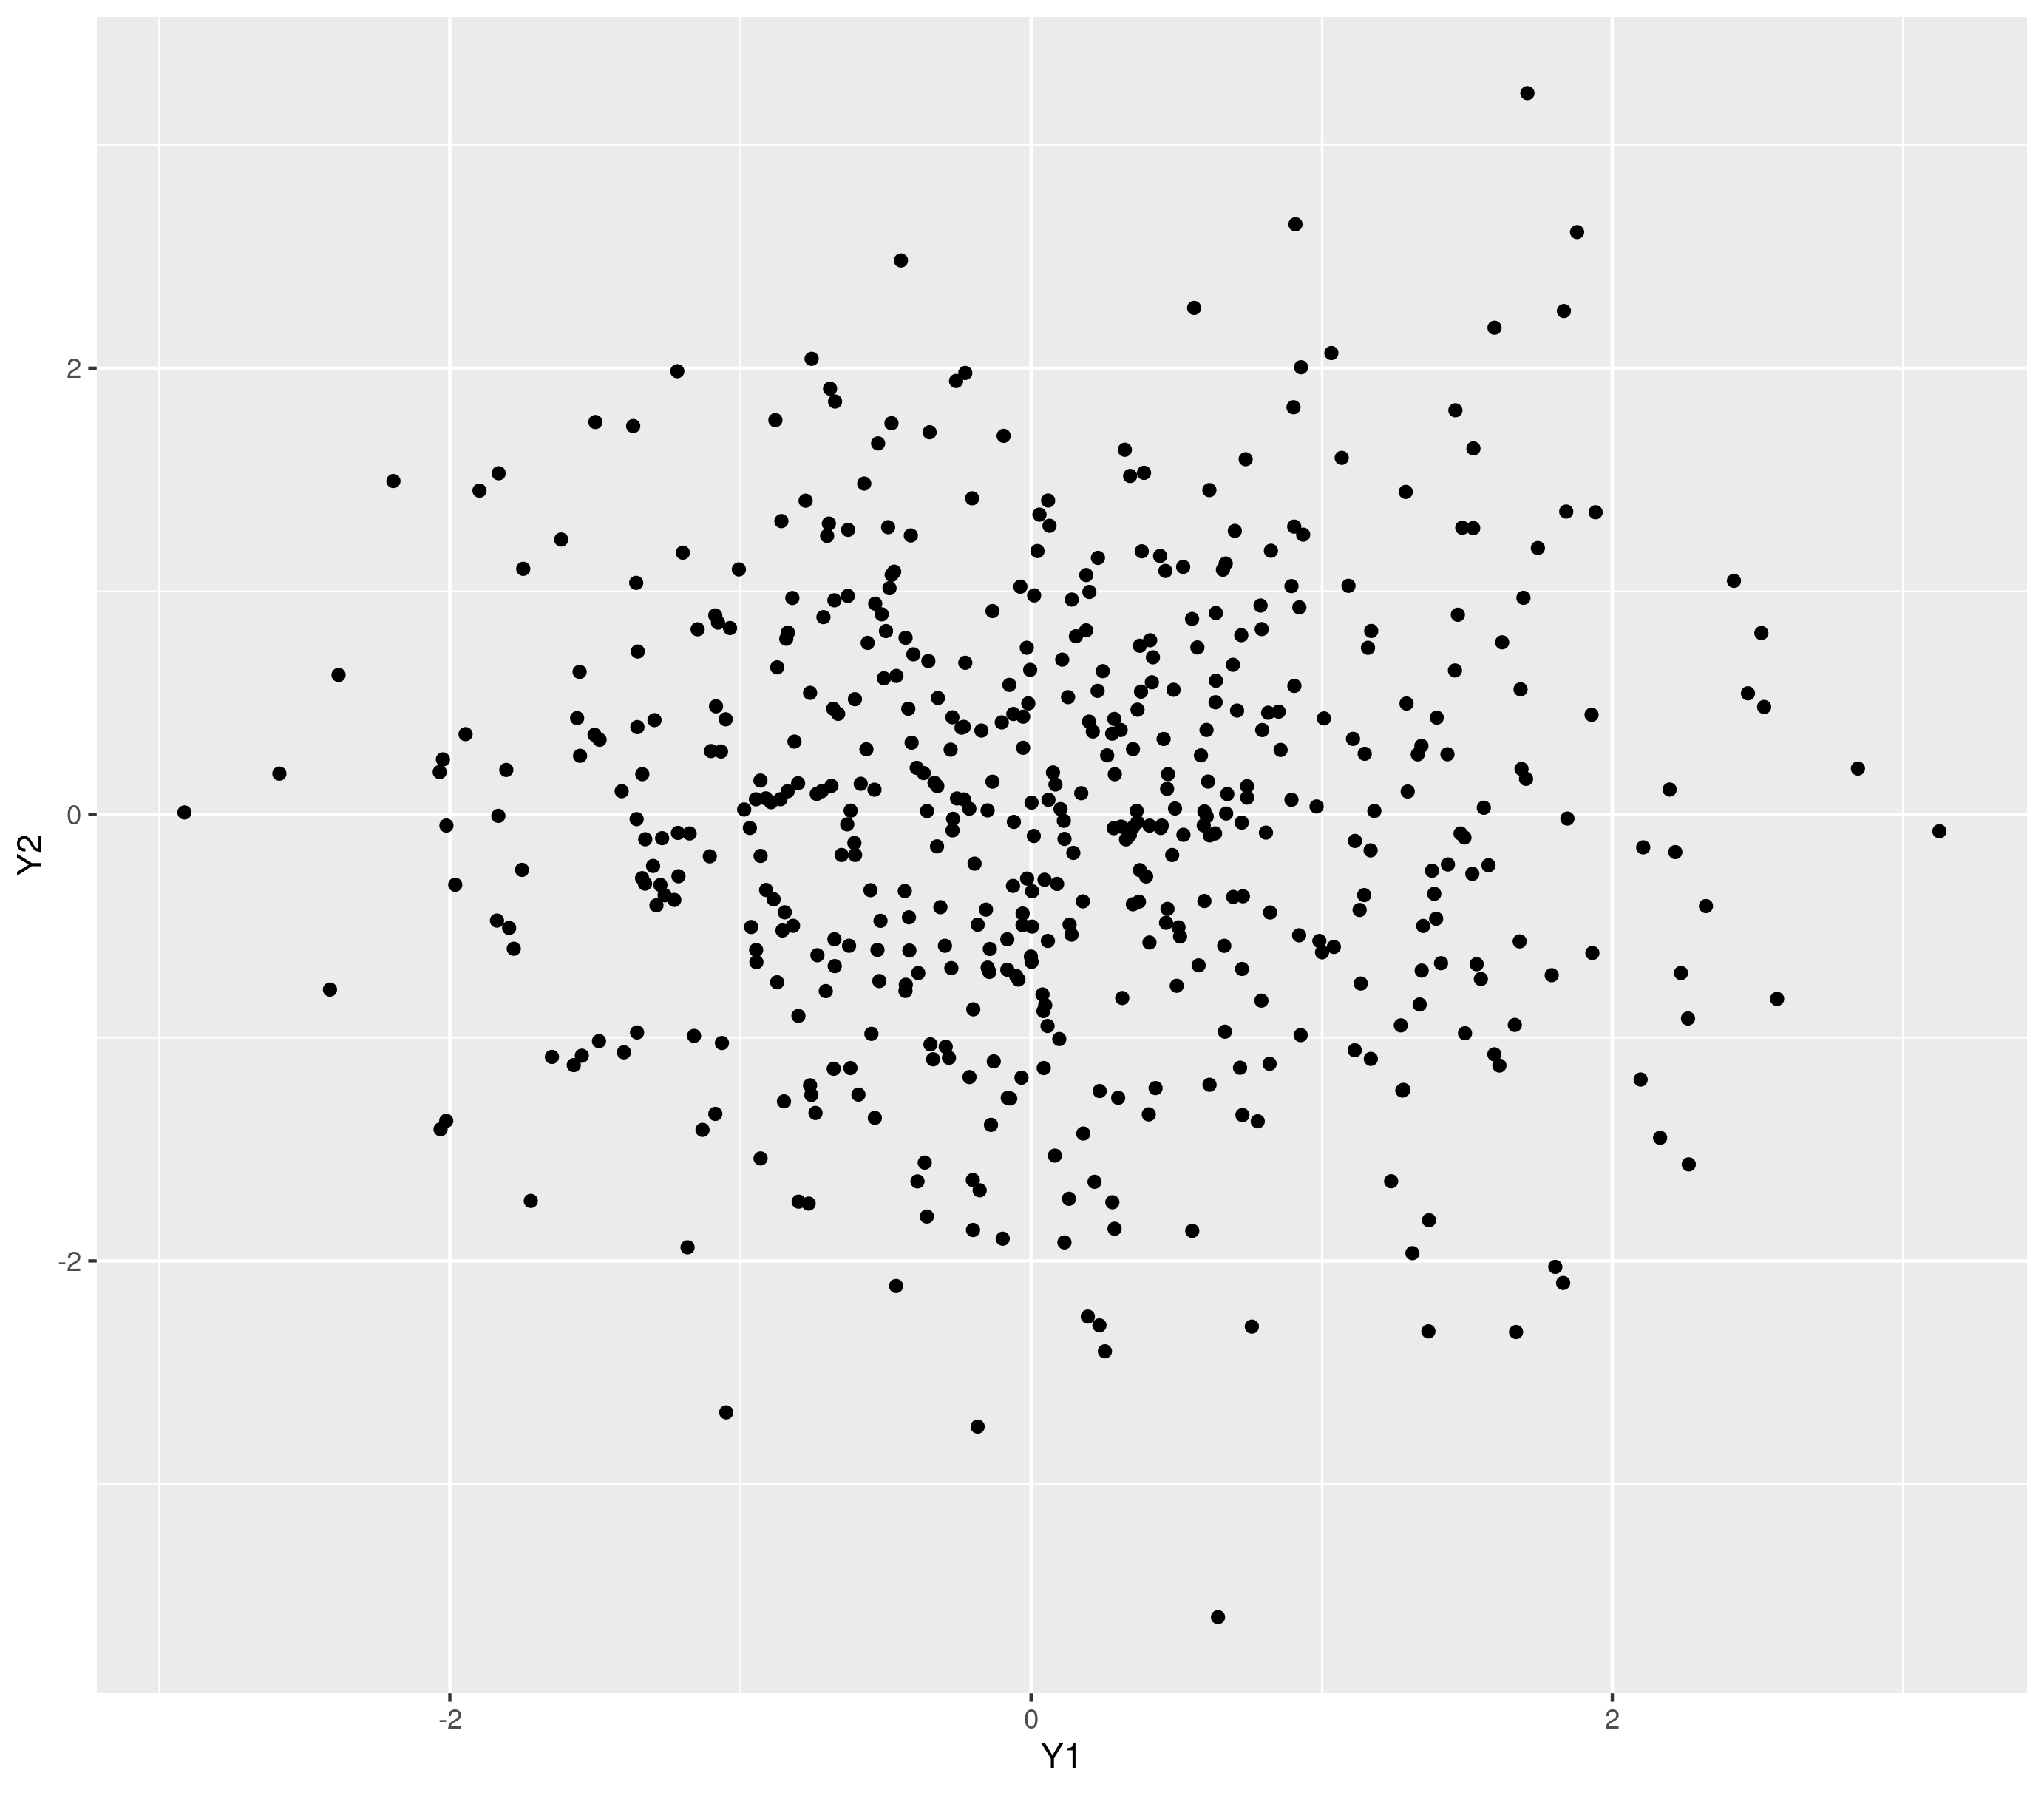
\includegraphics[scale=0.15]{bivariategaussian}}\\
      \only<2>{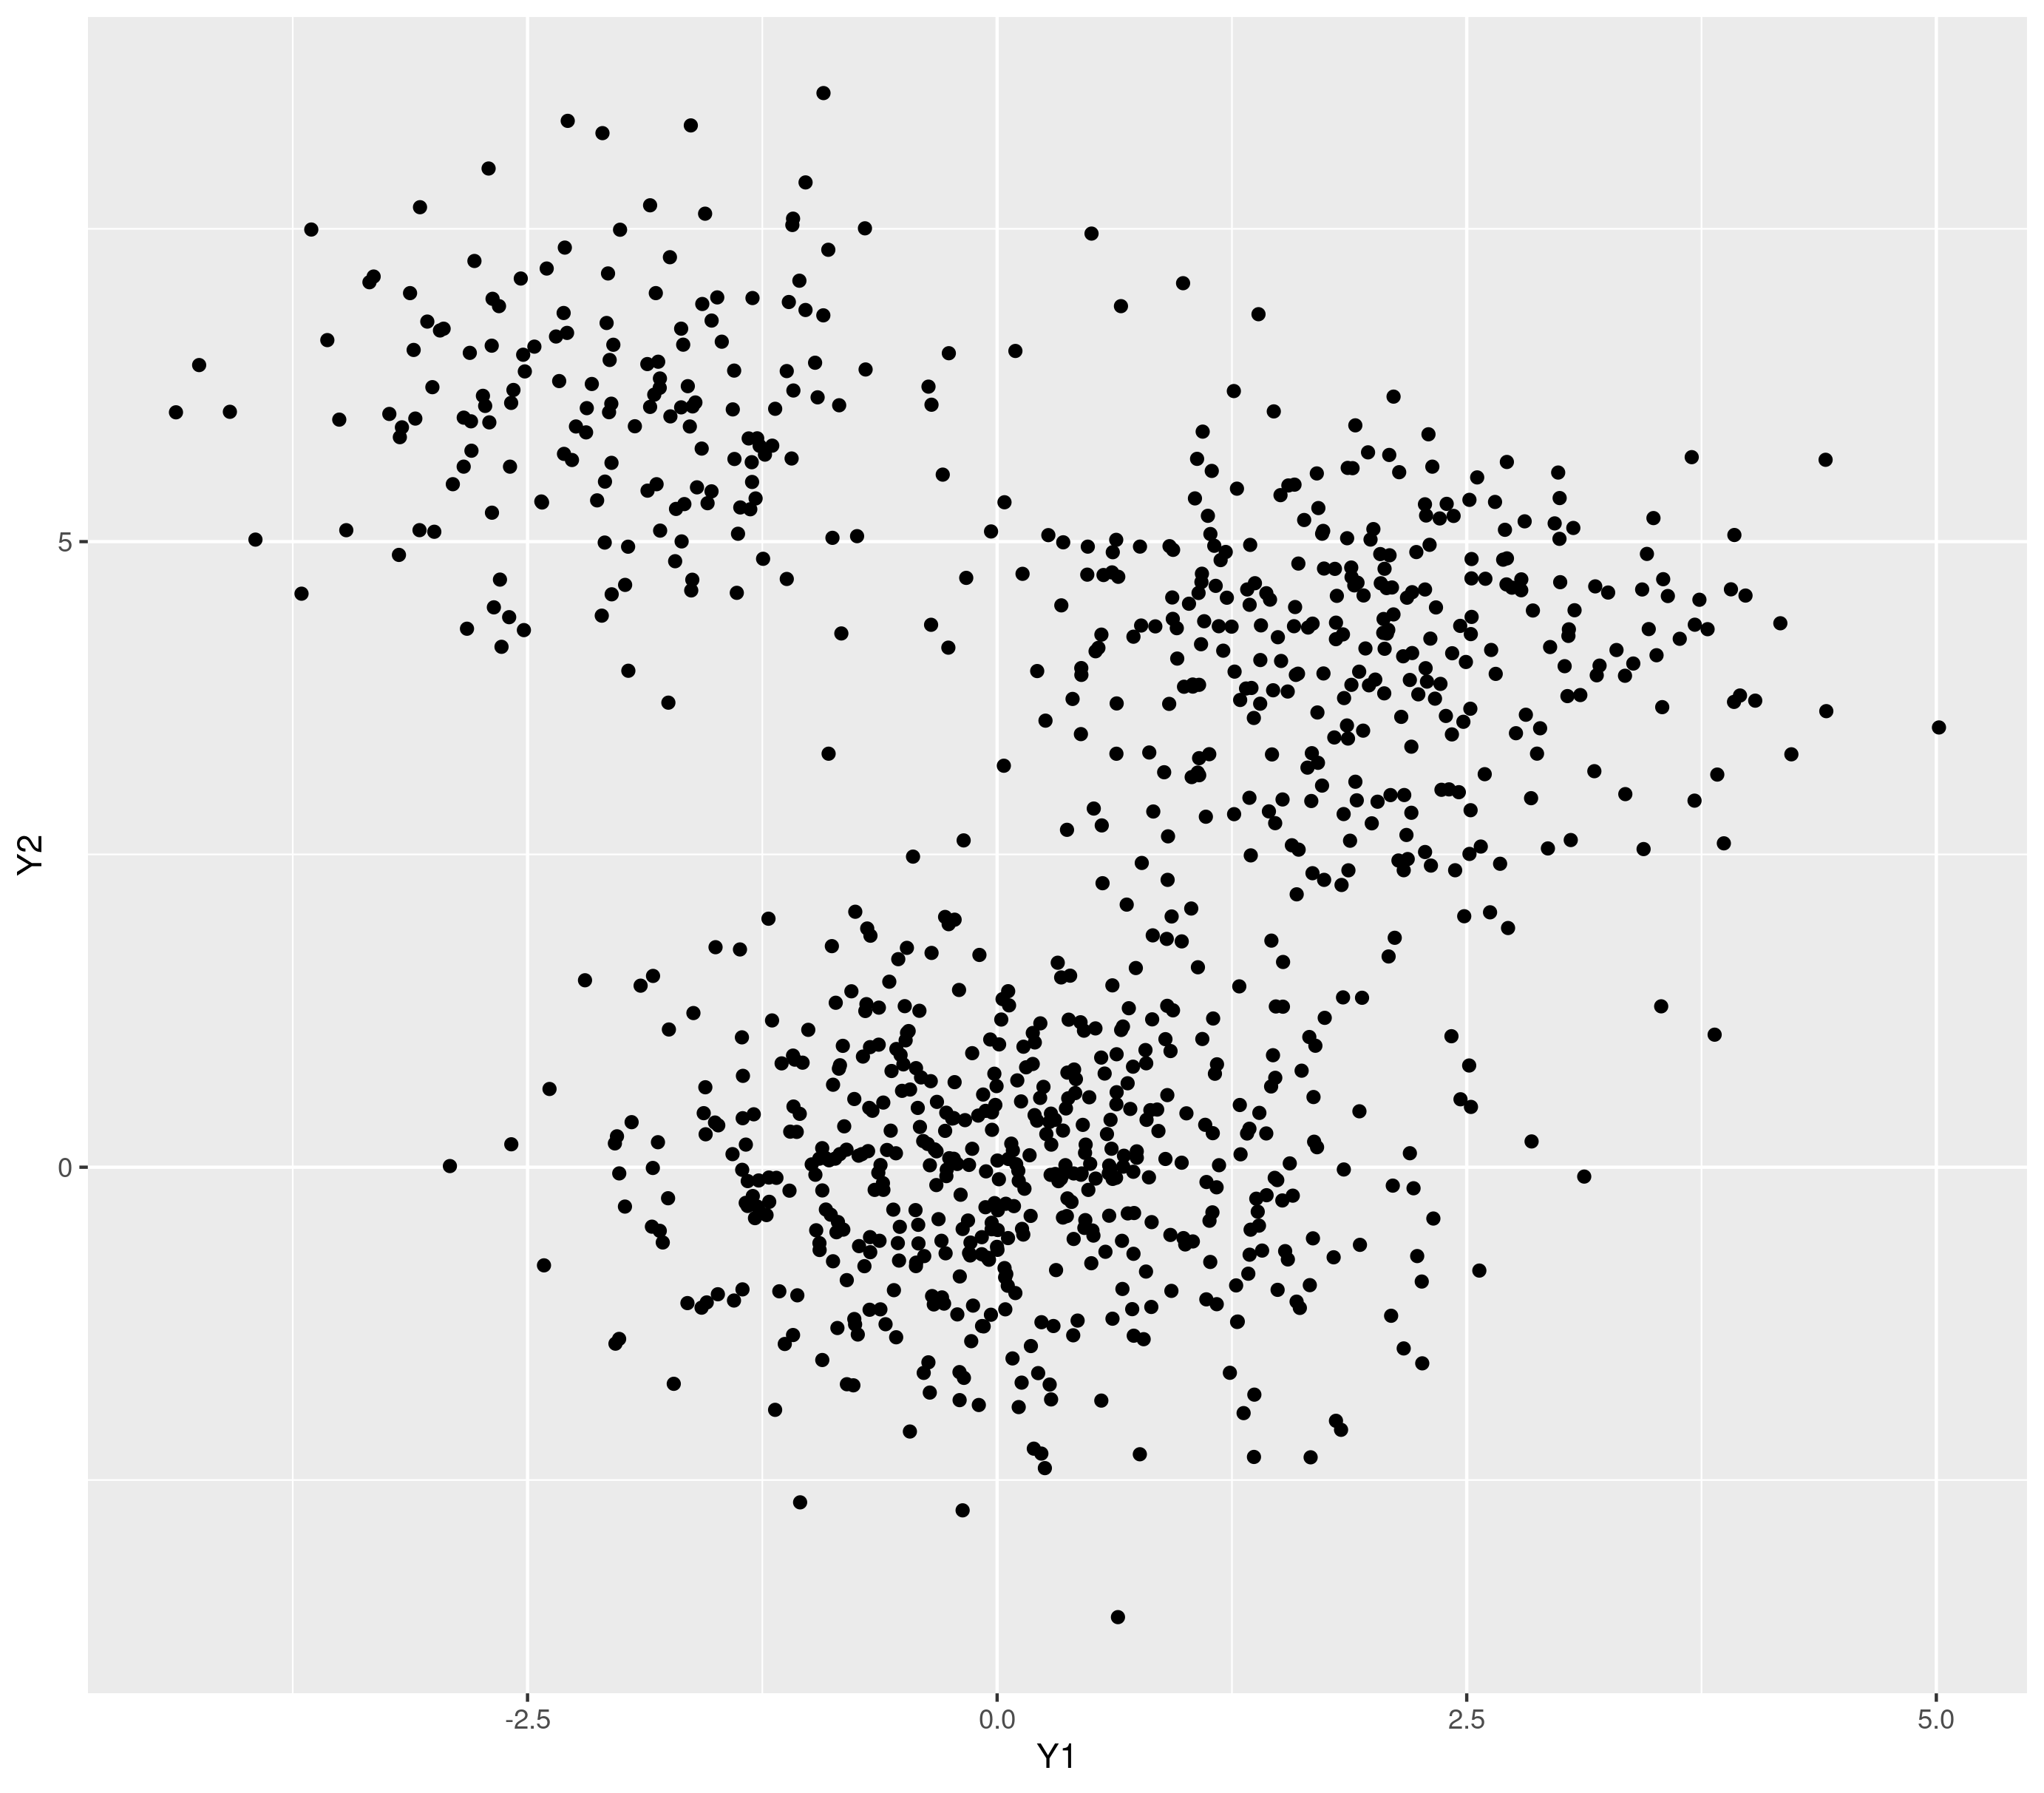
\includegraphics[scale=0.15]{bivariategaussianmixture}\\}
    \end{tabular}
  \end{center}
  
    \begin{itemize}
    \item[] \only<1> {Observation distribution seems easy to model with one Gaussian}
    \item[] \only<2> {Data are scattered and subpopulations are observed}
    \item[] \only<2> {According to the experimental design, there exists no external information about them}
    \end{itemize}
  
 \only<2> {\centerline{\textbf {This is an underlying structure observed through the data}}}
\end{frame}


%============================================
\begin{frame}{First  toy illustration}
%============================================

\begin{definition}[Mixture model]
It is a probabilistic model for representing the presence of subpopulations within an overall population.
\end{definition}
$$Y_i | Z_i = k  \sim \mathcal{N}(\mu_k,\Sigma_k), \quad  P(Z_i = k) = \pi_k
$$

\vspace{-1em}

\begin{tabular}{c|c|c}
   \tiny{what we observe} & \tiny{the model} &  \tiny{the expected results}  \\
   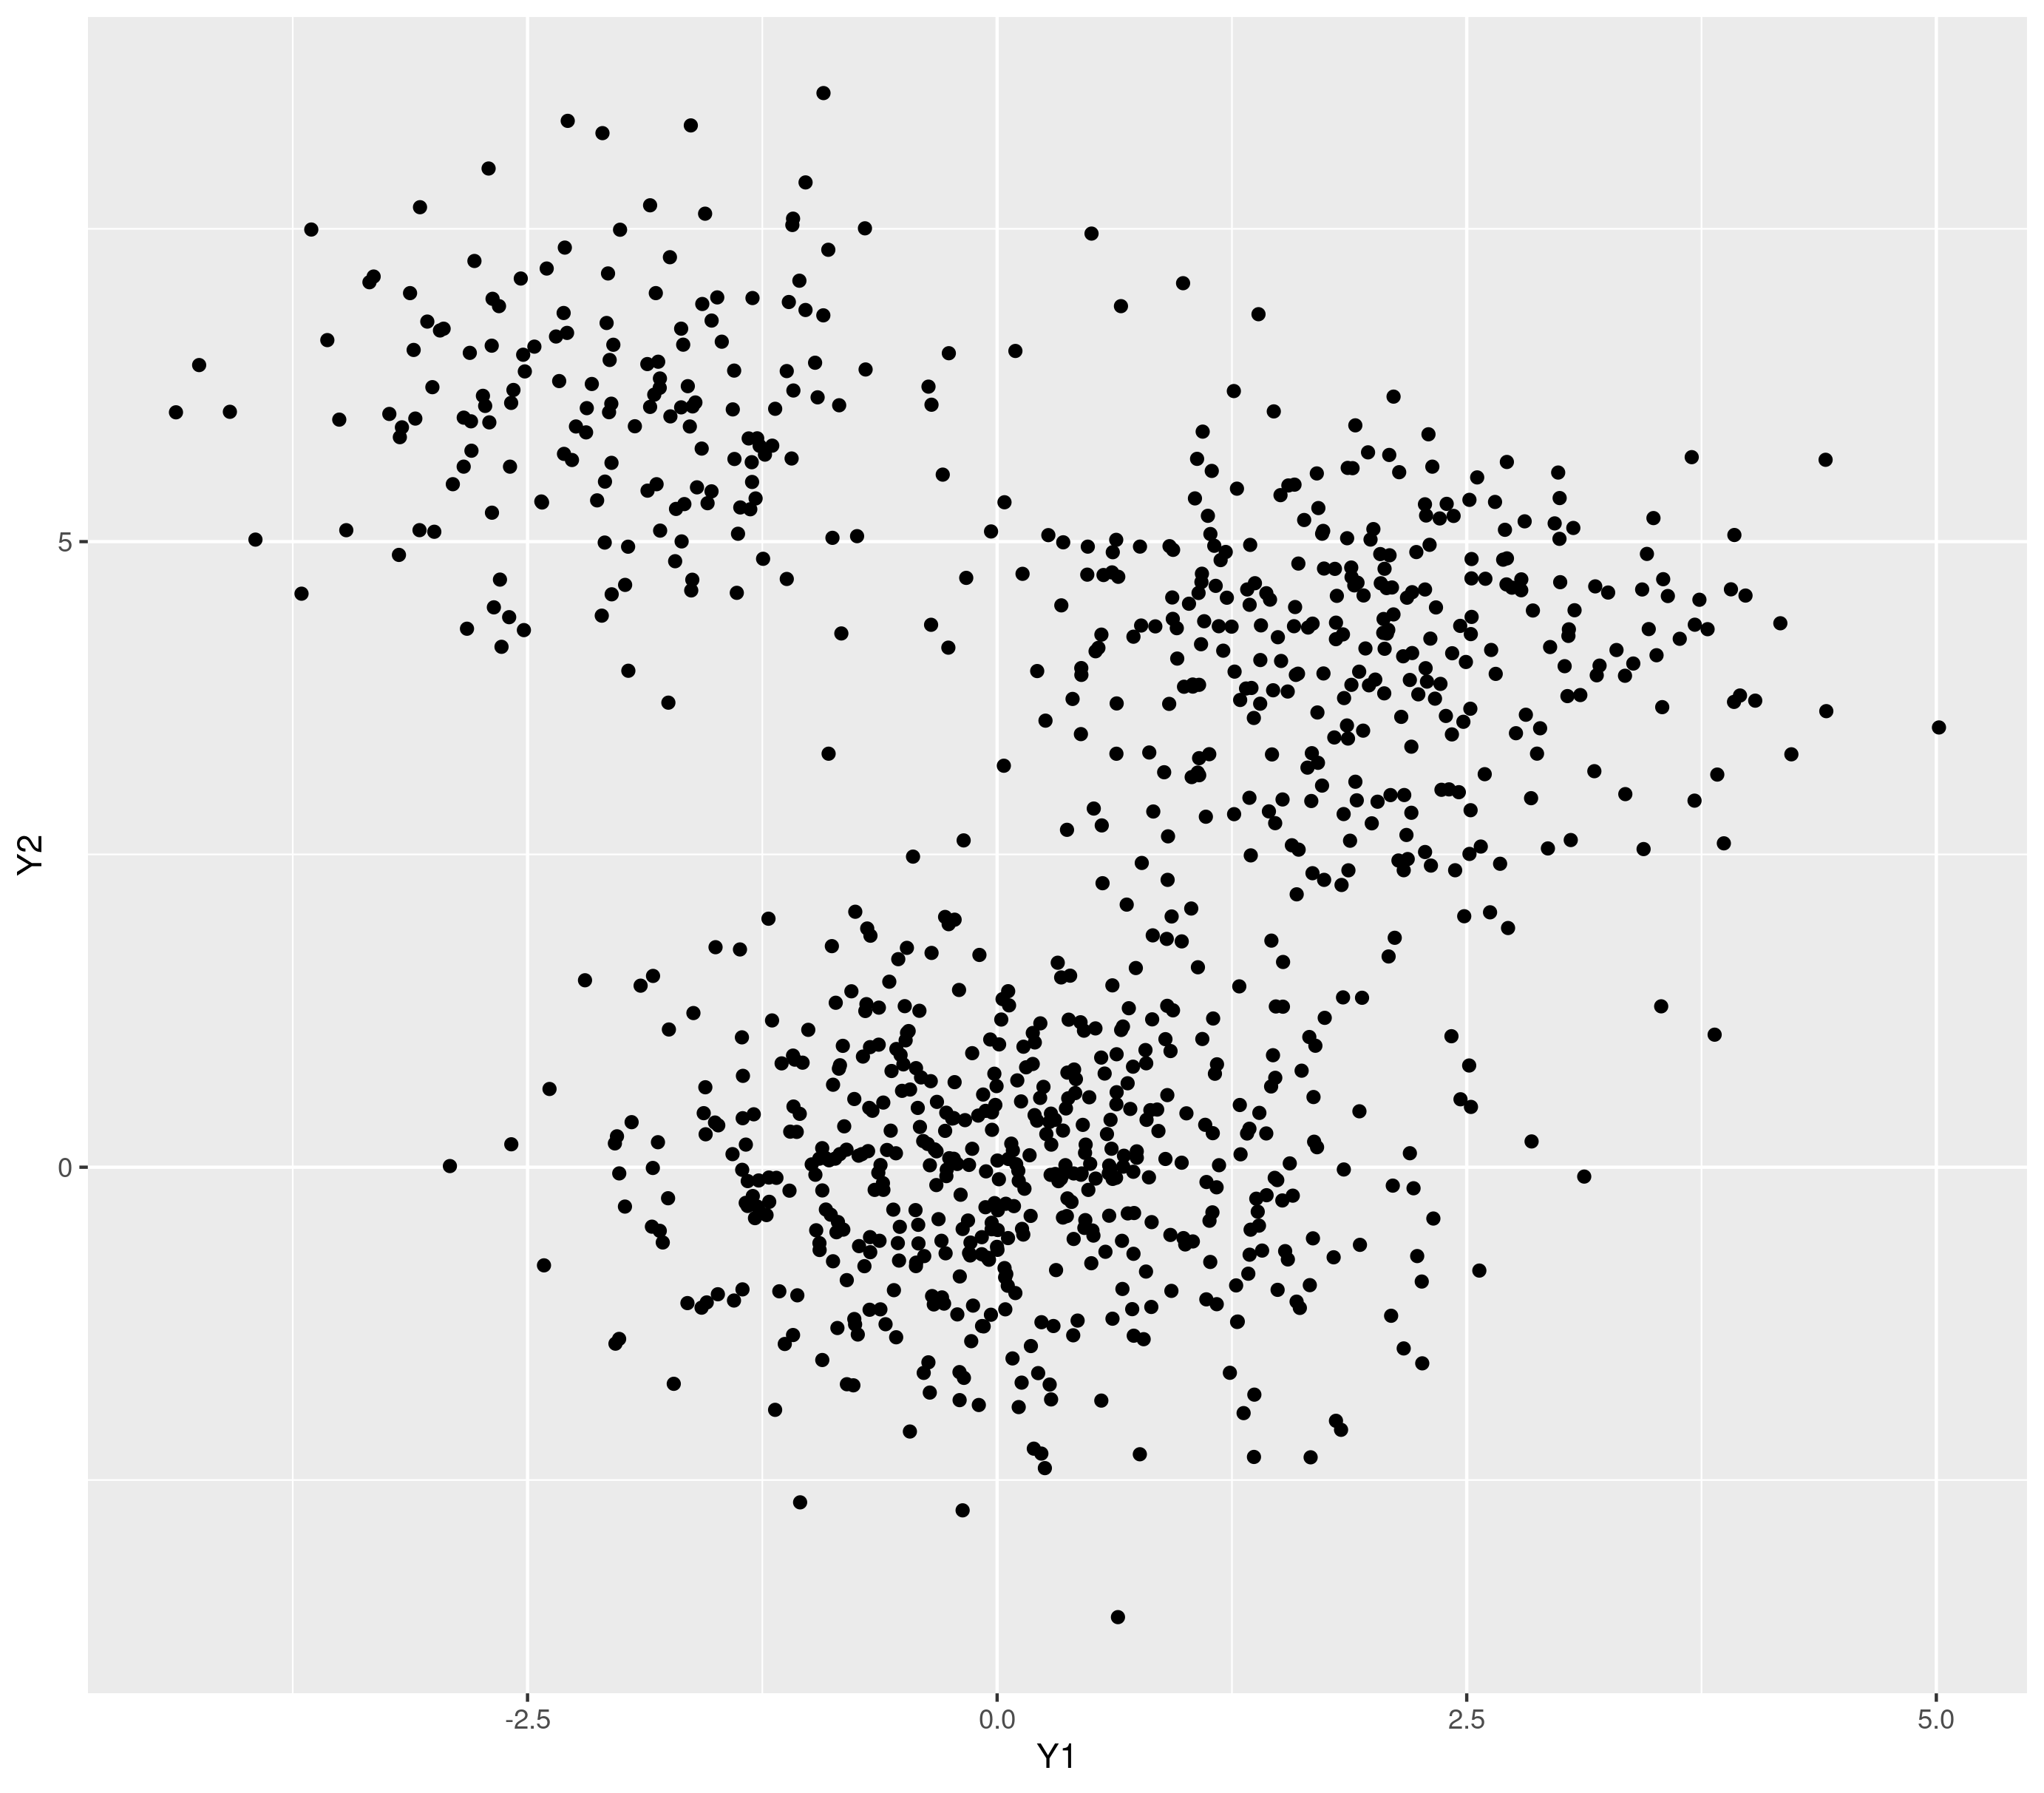
\includegraphics[scale=0.13]{bivariategaussianmixture}
  &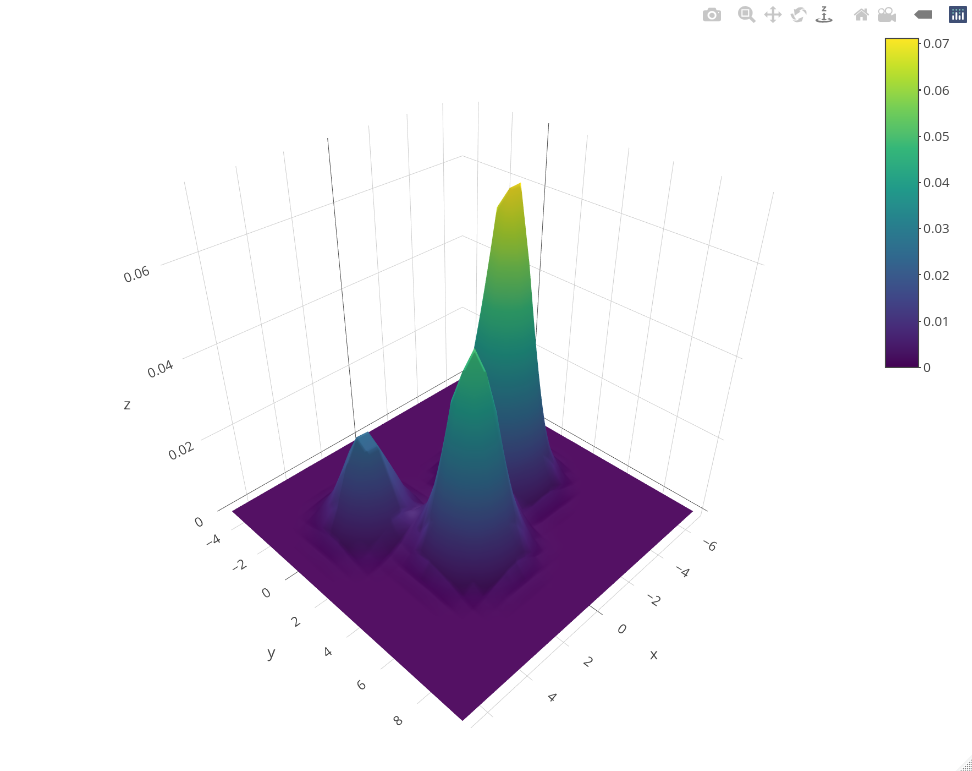
\includegraphics[scale=0.13]{bivariategaussianmixtureDensity}
  & 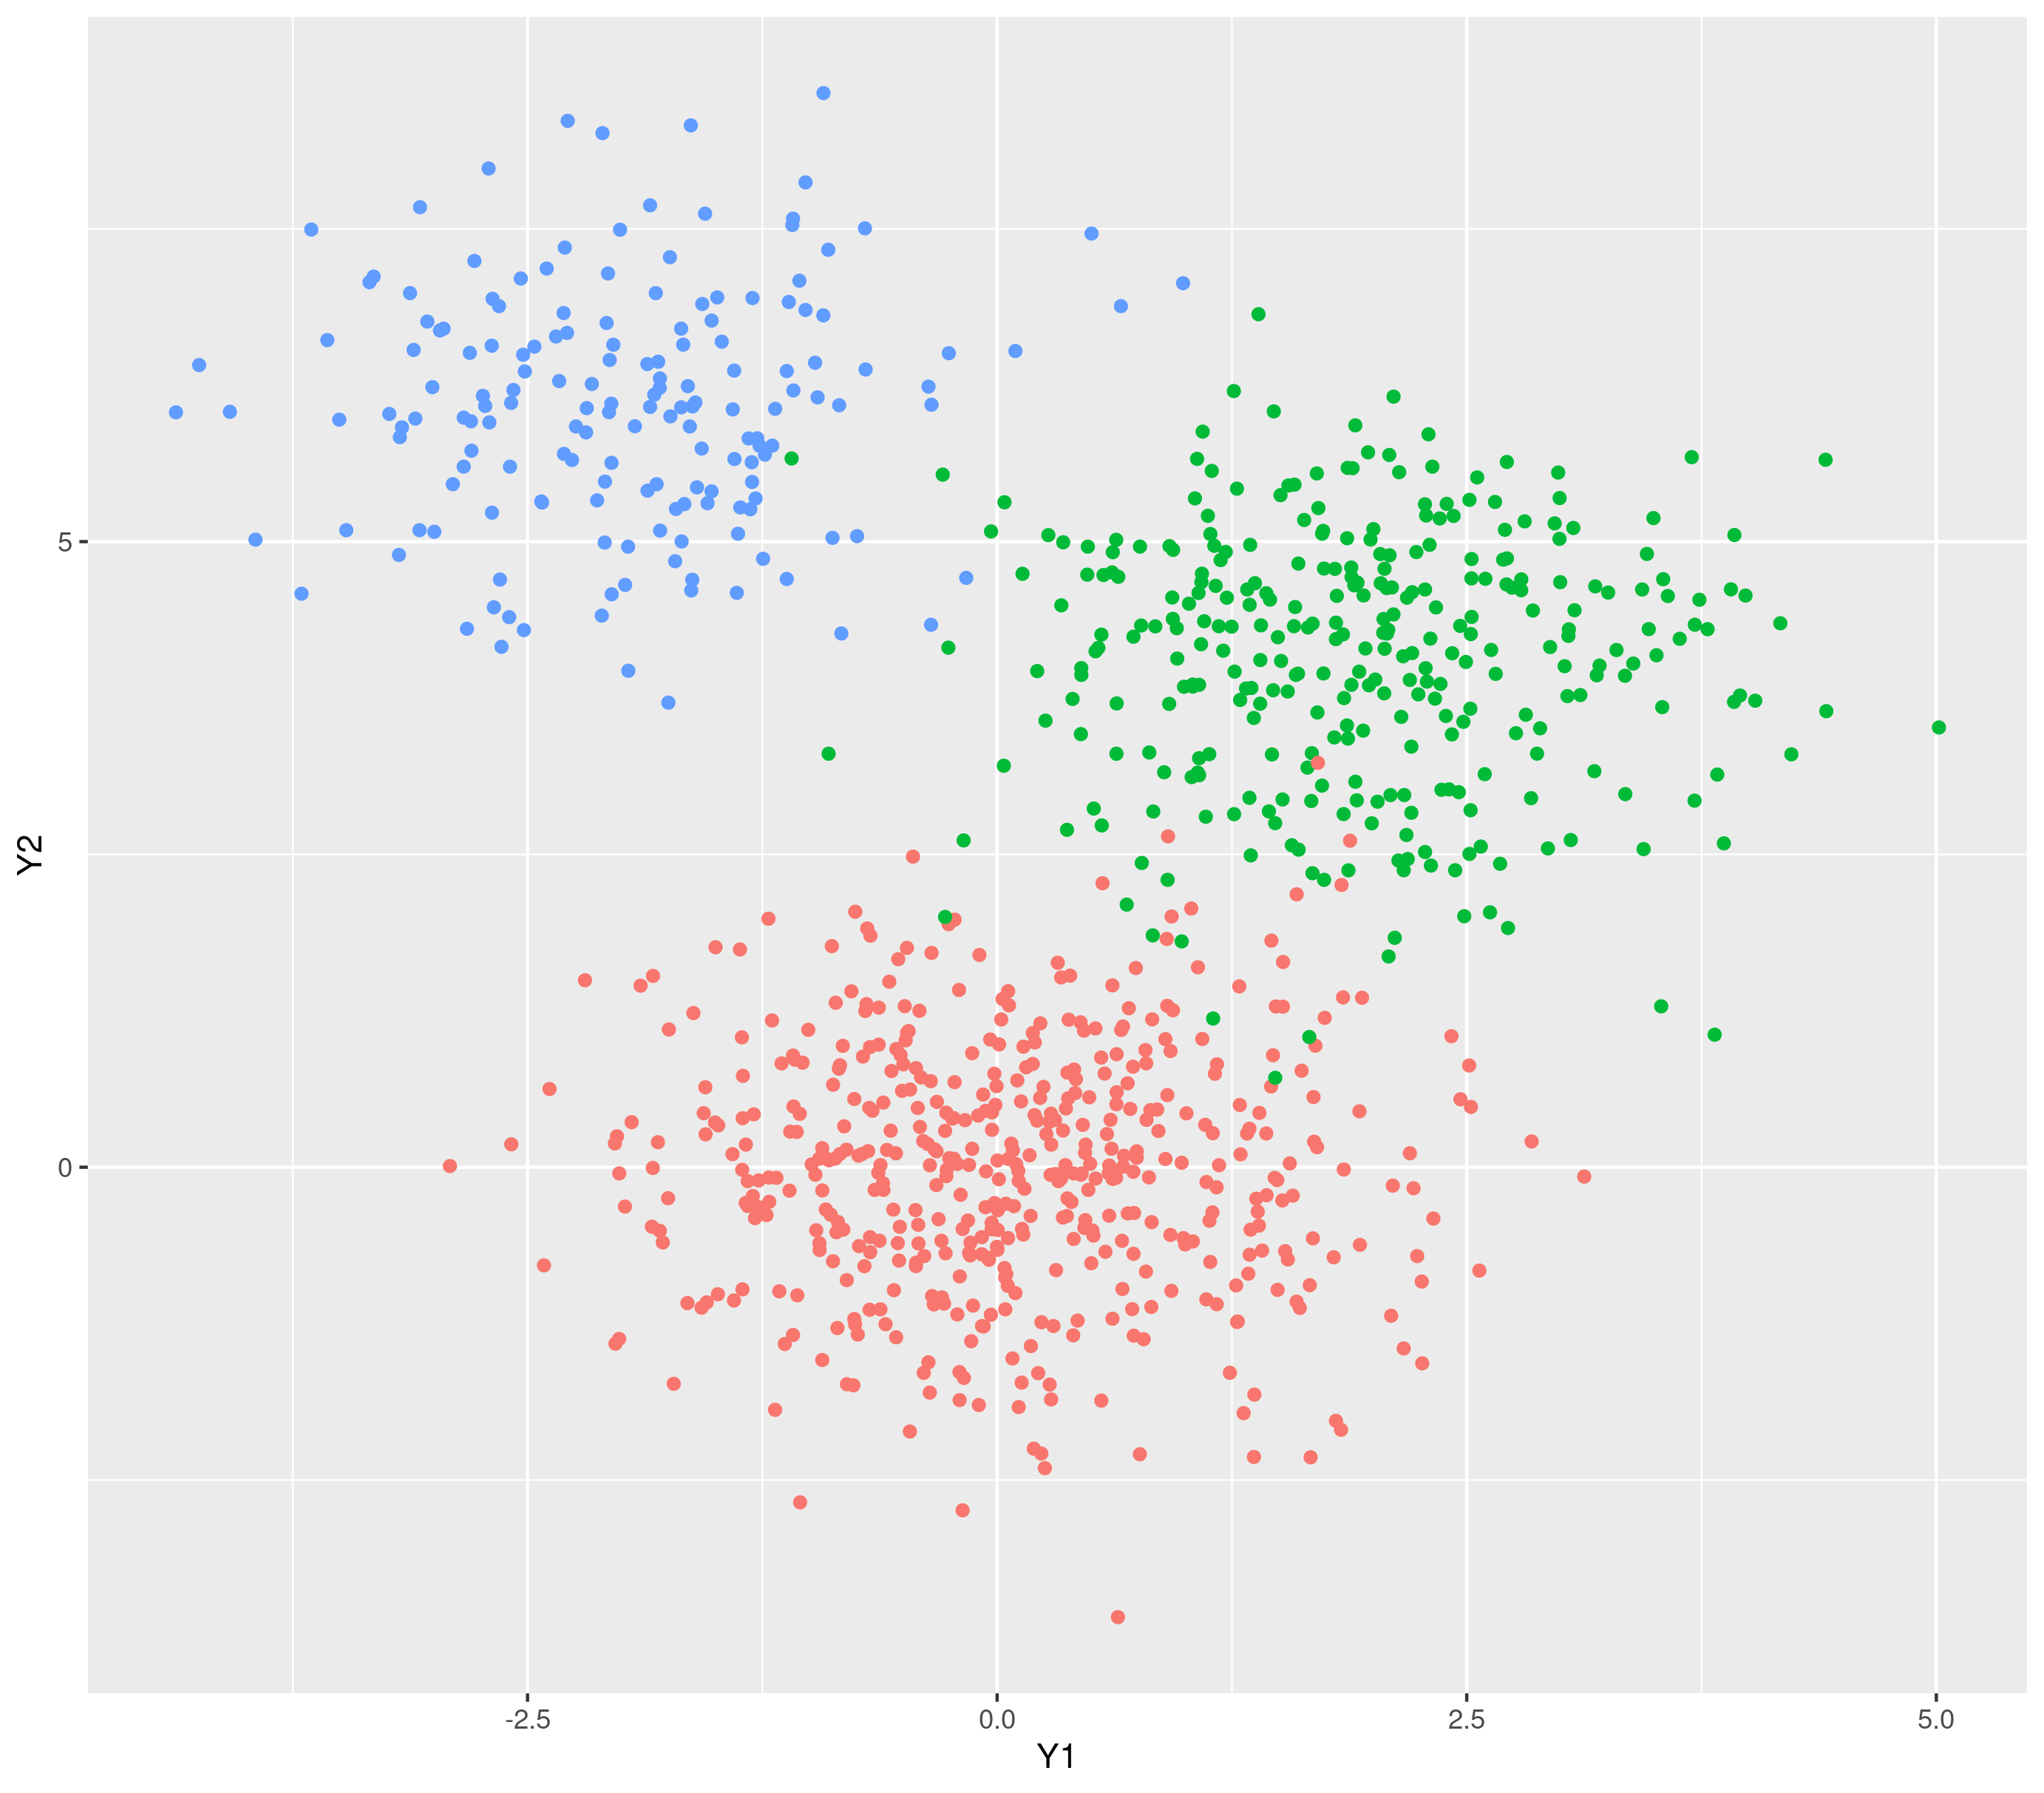
\includegraphics[scale=0.13]{bivariategaussianmixtureLabelled}\\
 &  & \\
  $Z =$ ? &
  & $Z: 1 = \textcolor{blue}{\bf \bullet}, 2 = \textcolor{red}{\bf \bullet}, 3 = \textcolor{green}{\bf \bullet}$ \\
\end{tabular} 

\vspace{1em}

\centerline{$\rightarrow$ It is an unsupervised classification method}
\end{frame}

%============================================
\begin{frame}
%============================================

\begin{itemize}
 \item Mixture model:  one of the most simple latent variable models
 \item \textcolor{dgreen}{Assumptions}
 \begin{itemize}
 \item Observations supposed to be independent, 
 \item Each  observation arises from a given class that is \textcolor{dgreen}{unobserved}
\end{itemize}
\item \textcolor{dgreen}{Main goal} : retrieve the class from which each observation arises
\item Also referred as  \textcolor{dgreen}{unsupervised classification} as we do not dispose of any observation with known label.
\end{itemize}
 
\end{frame}


% %===================================================
% \begin{frame}[allowframebreaks]{Gene expression}
% %===================================================
% 
% \begin{itemize}
%  \item To build groups of genes with related expression patterns (also known as coexpressed genes). 
%  \item Often such groups contain functionally related proteins, such as enzymes for a specific pathway, or genes that are co-regulated.
%  \item $Y_{tm}$ gene expression of gene at locus $t$ in condition $m = 1, \dots, P$ conditions. 
% \end{itemize}
% 
% \begin{center}
% 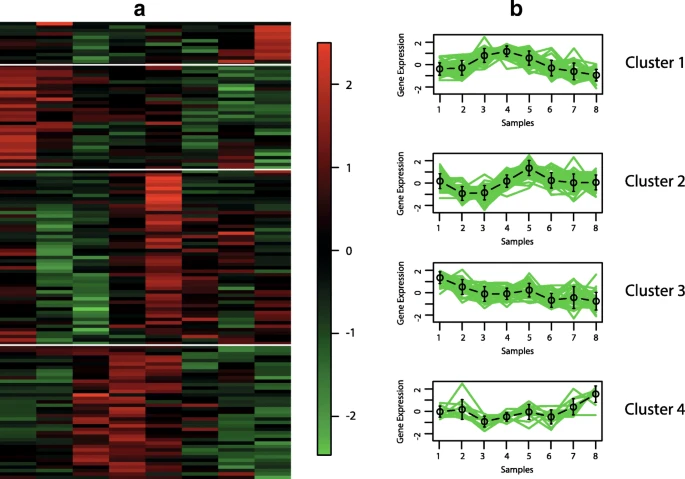
\includegraphics[scale = 0.35]{geneExpression}   
% \end{center}
% Figure from \cite{Parraga-Alava2018}
% \end{frame} 
%  




%==================================================
\begin{frame}{Applications in ecology}
%===================================================
\cite{rs13101989}
\emph{Gaussian mixture model to separate Birds and Insects in Single-Polarization Weather Radar data}

\begin{itemize}
 \item Use of weather radar data to quantify to flow of nocturnal bird migration
 \item Methods distinguish well between precipitation and  birdsbut not well between birds and insects
\end{itemize}\centering
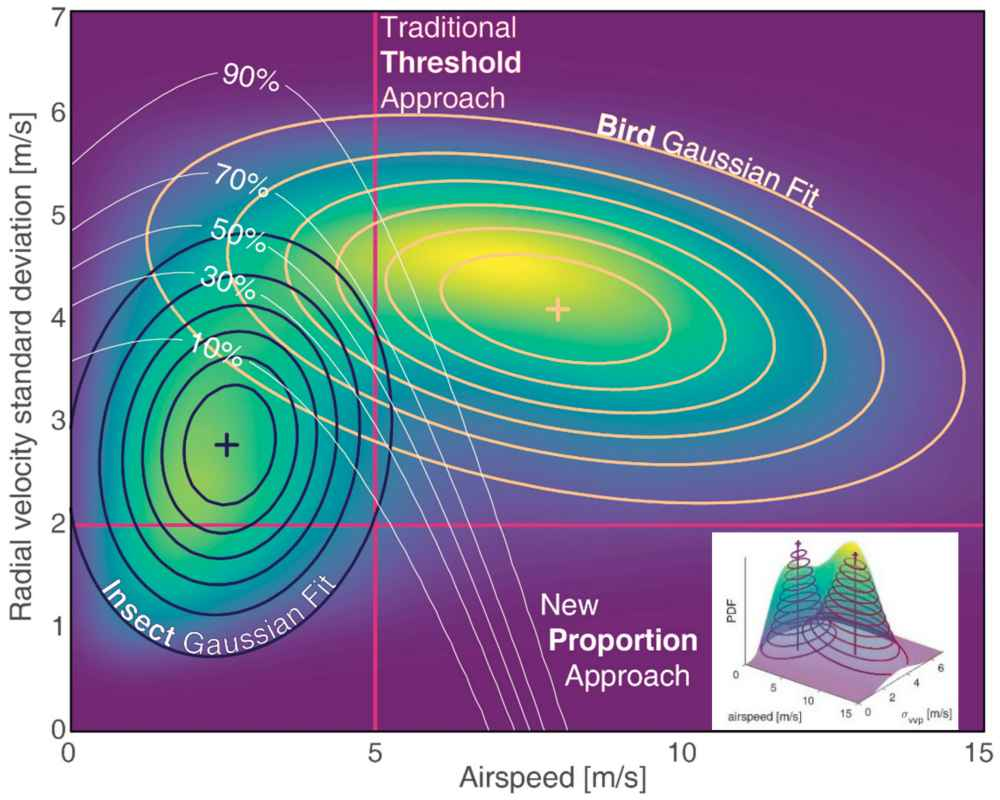
\includegraphics[scale=0.13]{WeatherRadar}
\end{frame}
%  

%===================================================
\begin{frame}[allowframebreaks]{Plant and animal ecology}
%===================================================

To describe and to make spatial and temporal comparisons of communities (assemblages) of organisms in heterogeneous environments.
 
 
\begin{itemize}
 \item $Y_{is}$: abundancy of species $i$ at location $s$.
 \item Not the same repartitions with respect to species. 
\end{itemize}



\begin{center}
  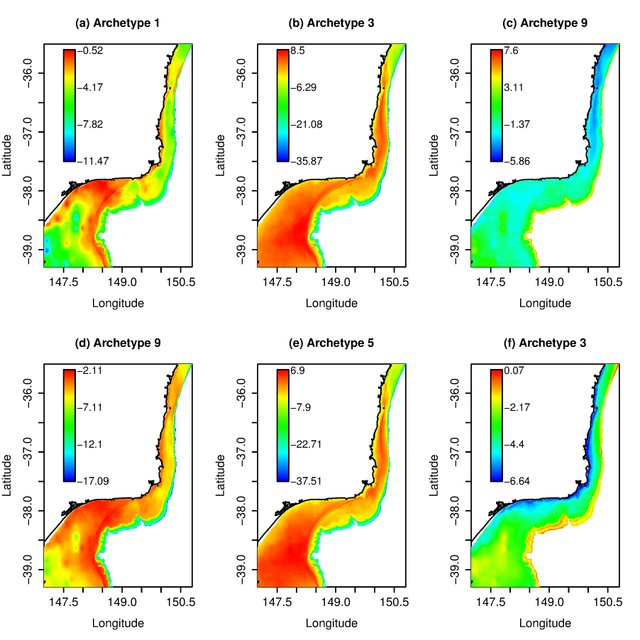
\includegraphics[scale = 0.27]{ecology_spatial_archetypes}   
\end{center}
     
\cite{Dunstan2013}


\end{frame}


%===================================================
\begin{frame}{Human genetic}
%===================================================

\begin{itemize}
 \item Better understand the genetic structure of populations
 \item Relies on the genotyping of large sets of individuals sampled in different places, environments or with different origins
 \item Genotype $Y_{it}$ of a series of individuals $i \in \interval{1}{I}$ at a series of locus $t \in \interval{1}{T}$ is measured
 \item \textcolor{dgreen}{Aim}: distinguish sub-populations.
\end{itemize}

\end{frame}
%===================================================
\begin{frame}{Model without 'admixture'}
%===================================================

Each individual $i$ is supposed to belong to one population, labeled $Z_i$

 \begin{eqnarray*}
 (Z_i)_i \text{ iid} & \sim & \Mcal(1; \pi), \\
 (Y_{it})_{i, t} \text{ indep.} \,|\, (Z_i) & \sim & \Mcal(2; \gamma_{Z_it}),
\end{eqnarray*}
$\gamma_{kt}$ is the vector of the allelic frequencies at locus $t$ in population $k$

which makes explicit the fact that, if individual $i$ belongs to population $k$, its genotype is generated with the allelic frequencies of its population.
\end{frame}



%===================================================
\begin{frame}{Model with  'admixture'}
%===================================================
\begin{eqnarray*}
 (Y_{it})_{i, t} \text{ indep.} \,|\, (Z_i) & \sim & \Mcal(2; \gamma_{Z_it})\\
 (Z_i)_i \text{ iid} & \sim & \Mcal(1; \pi_i), \\
\pi_i  & \sim & \mathcal{D}(1; \alpha)
\end{eqnarray*} 

\textbf{About $\pi_i$}: individual preferential trends characterized
\begin{itemize}
  \item Dirichlet distribution whose support is the the simplex of $\mathbb{R}^K$.
 \item $\pi_i$ is the position of individual $i$ in the simplex, the vertices of which correspond to fictitious individuals purely issued from each population. 
 \end{itemize}
 
Hidden variable is hence $ (Z_i, \pi_i)$. 
\end{frame}
 

 
%===================================================
\begin{frame}{Model with  'admixture': reformulation}
%===================================================

The model can be rewritten also after marginalization over $Z_{it}$:
\begin{eqnarray*}
 (\pi_i)_i \text{ iid} & \sim & \mathcal{D}(1; \alpha), \\
 (Y_{it})_{i, t} \text{ indep.} \,|\, (\pi_i) & \sim & \Mcal\left(1;\sum_k \pi_{ik} \gamma_{kt}\right).
\end{eqnarray*} 
The latent variable reduces then to $(\pi_i)$.


See \cite{Pritchard2000} for more details. 
\end{frame}

%===================================================
\begin{frame}{Expected results}
%===================================================

\begin{center}
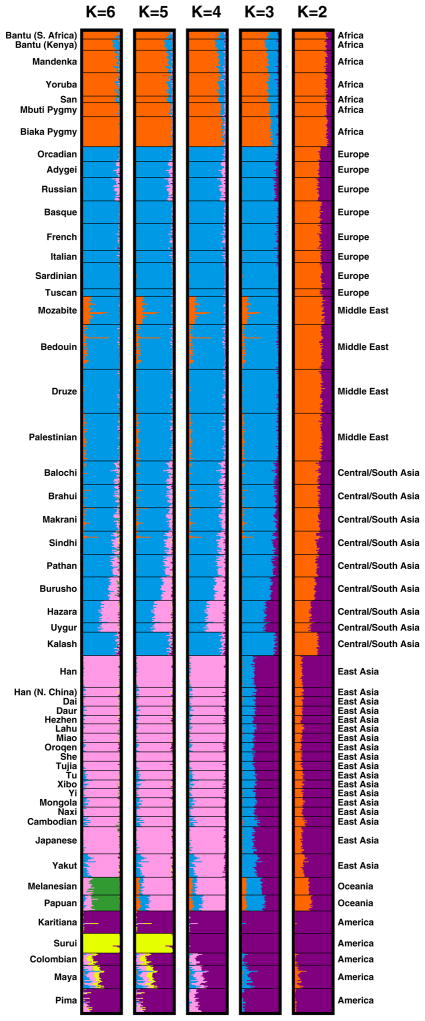
\includegraphics[angle=90, scale = 0.6]{nihms426502f6}   
\end{center}

Population origine of series of human genomes with varying number of groups $K$. Each column corresponds to an individual. 
Each individual is represented by a thin vertical line partitioned into K colored segments that represent the fractions of the individual’s genome estimated to belong to the K clusters.
From \cite{Rosenberg11}. 


\end{frame}

 
 


 


%===============================================
\section{The mixture model}
%==============================================

\subsection{Definition}
%===============================================
\begin{frame}{Definition}
%=============================================== 
\begin{itemize}
 \item Let $(Y_i)_{i=1,\dots, n}$ be independent variables 
\item For each individual $i$ assumes the existence an unknown (or latent) label $Z_i$ that can take a finite number of values among $\interval{1}{K}$. 
\item The distribution of  $Y_i$ depends on the value  $Z_i$. 
 \end{itemize}


\begin{definition} \label{Def:MixtureModel}
  An independent $K$ mixture model is defined as follows: $\forall i =1,\dots,n$
  \begin{equation} \label{Eq:MixtureModel}
  \begin{array}{ccl}
  \Prob(Z_i = k) & = &  \pi_k,  \quad \quad \quad (i.i.d)\\
  Y_i | (Z_i = k) & \sim_{i.i.d}& \Fcal_k = \Fcal(\gamma_k),
  \end{array}
  \end{equation}
  where $\sum_{k=1}^K\pi =1$. 
\end{definition}


Let  $f_k(\cdot) = f(\cdot; \gamma_k)$ be the pdf of distribution of  $\Fcal(\gamma_k)$.

\end{frame}

%===============================================
\begin{frame}{Alternative fomulations}
%=============================================== 
\begin{itemize}
 \item
 $
Y_{i}| (Z_i = k) \sim \Fcal(\gamma_{k}) 
$
is equivalent to
$
Y_{i} | Z_i \sim \Fcal(\gamma_{Z_i})
$
\item Let $Z_{ik} = \ind_{\{Z_i=k\}}$
$$(Z_{ik})_{k=1,\dots,K} \sim \Mcal(1,\bpi)$$
where $\Mcal$ is the \href{https://en.wikipedia.org/wiki/Multinomial_distribution}{multinomial distribution} $\bpi = (\pi_1, \dots,\pi_K)$
\end{itemize}


\end{frame}
%=============================================== 
\begin{frame}{About the mixture proportions}
%=============================================== 
\begin{itemize}
  \item $\pi_k =$ proportion of the population $k$
  \item Sometimes called \textcolor{dgreen}{prior probabilities} although this denomination may be misleading in a non-Bayesian context. 
 \item Also often refereed to as the \textcolor{dgreen}{proportions} of the mixture.
\end{itemize}
\end{frame}

%=============================================== 
\begin{frame}{About the emission distribution}
%===============================================
\begin{itemize}
\item Conditionally on   $\{Z_i = k\}$, $Y_i$ has a parametric distribution $\Fcal_k = \Fcal(\gamma_k)$ with probability distribution function (pdf) $f_k(\cdot) = f(\cdot; \gamma_k)$.
\item  $\Fcal_k$ is called the \textcolor{dgreen}{emission} distribution in class $k$ \item It describes how observed data arising from class $k$ are emitted. 
\item $f_k$ is called the emission pdf.
\end{itemize}
\end{frame}


 \subsection{Properties}
 
%=============================================== 
\begin{frame}{Other formulation}
%=============================================== 
\textbf{\color{dgreen} Useful notations}
\begin{itemize}
 \item $\bZ = (Z_1, \dots, Z_n)$
 \item $\bY  = (Y_1,\dots, Y_n)$
 \item $\bpi = (\pi_k)_{k=1, \dots,K}$
 \item $\bgamma = (\gamma_k)_{k=1, \dots,K}$
 \item $\theta  = (\bpi,\bgamma)$
\end{itemize}

\vspace{2em}

\textbf{\color{dgreen} Conditional distributions}

$$
\begin{array}{cclcll}
   p_\theta(\bZ) & = &  \prod_{i=1}^n \pi_{Z_i} &=&  \prod_{i=1}^n \prod_{k=1}^{K}  (\pi_k)^{Z_{ik}}, \\
  p_\theta(\bY|\bZ) & = & \prod_{i=1}^n f(Y_i, \gamma_{Z_i})  &=& \prod_{i=1}^n \prod_{k=1}^{K} f(Y_i, \gamma_k)^{Z_{ik}}, 
\end{array}
$$
\end{frame}

%=============================================== 
\begin{frame}{Marginal distribution}
%=============================================== 
 Marginal pdf.  of $Y_i$ is the mixture distribution
$$
g(y) = \sum_{k=1}^K \pi_k f(y; \gamma_k).
$$

 



\begin{columns}
\begin{column}{0.5\textwidth}
 Example of a mixture of $K=3$ Gaussian distributions
$\frac{1}{3}\mathcal{N}(1,1) + \frac{1}{6}\mathcal{N}(3,1) + \frac{1}{2}\mathcal{N}(5,3^2)$
\end{column}
\begin{column}{0.5\textwidth}
    \begin{center}
   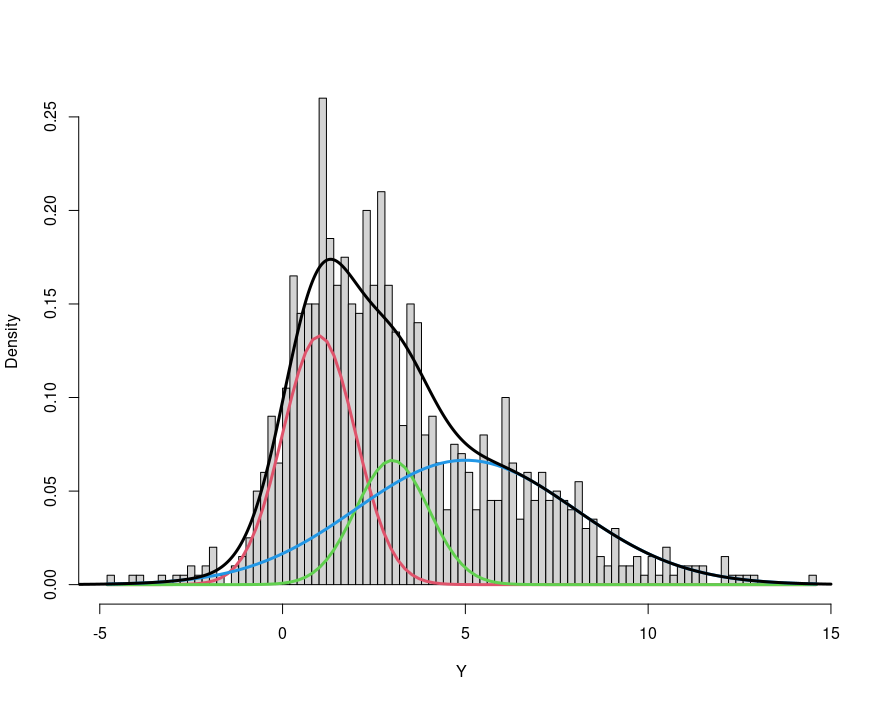
\includegraphics[width=\textwidth]{gaussian_mixtures}   
     \end{center}
\end{column}
\end{columns}
\end{frame}

%=============================================== 
\begin{frame}{Label switching}
%=============================================== 


Since the $(Z_i)$ are not observed, the model is invariant for any permutation of the labels $\interval{1}{K}$. 

Therefore, the mixture model with $K$ classes has $K!$ equivalent definitions.
\end{frame}


%=============================================== 
\begin{frame}{Number of parameters}
%=============================================== 
\begin{itemize}
 \item Depends on both the dimension of the data and the number of groups
  \item $\sum_{k=1}^K \pi_k = 1$, $\bpi$ involves only $K-1$
  \item About $\bgamma = (\gamma_1, \dots, \gamma_K)$, its dimension is typically proportional to the number of groups $K$
  \item For \textcolor{dgreen}{$\Fcal_k$: univariate Poisson distributions with respective mean $\gamma_k$ } , $\bgamma$ of dimension $K$ $\Rightarrow$ $2K-1$ parameters
 \item For \textcolor{dgreen}{$\Fcal_k$: $d$-variate normal distributions} (with respective mean vector $\mu_k$ and variance $\Sigma_k$): $$(K-1) + Kd + Kd(d+1)/2 \simeq Kd^2/2$$ parameters 
\end{itemize}
\end{frame}


%=============================================== 
\begin{frame}{Dependency structures}
%=============================================== 
 \begin{itemize}
 \item The $(Z_i)$ are independent;
 \item the $(Y_i)$ are independent conditionally to $\bZ = (Z_i)_{i=1,\dots,n}$;
\item the couples $\{(Y_i, Z_i)\}_i$ are iid.
 \end{itemize}
% 
 \begin{center}
 \begin{tikzpicture}
 \node[hidden] (Z1) at (0, 0) {$Z_1$};
 \node[hidden] (Zi) at (\edgeunit, 0) {$Z_i$};
 \node[hidden] (Zj) at (2*\edgeunit, 0) {$Z_j$};
 \node[hidden] (Zn) at (3*\edgeunit, 0) {$Z_n$};
 
 \node[observed] (Y1) at (0, -1*\edgeunit) {$Y_1$};
 \node[observed] (Yi) at (\edgeunit, -1*\edgeunit) {$Y_i$};
 \node[observed] (Yj) at (2*\edgeunit, -1*\edgeunit) {$Y_j$};
 \node[observed] (Yn) at (3*\edgeunit, -1*\edgeunit) {$Y_n$};
   
 \draw[arrow] (Z1) to (Y1);
 \draw[arrow] (Zi) to (Yi);
 \draw[arrow] (Zj) to (Yj);
 \draw[arrow] (Zn) to (Yn);
 \end{tikzpicture}
 
 Graphical representation of a mixture model
 \end{center}
\end{frame}


%=============================================== 
\begin{frame}{Remarks}\label{Rq:MixtureInd}
\begin{enumerate}
\item Because the $\{(Y_i, Z_i)\}_i$ are independent, we have that
  $$
  p_\theta(Z_i |\bY) = p_\theta(Z_i | Y_i)
  $$
  which means that the information about the classification of individual $i$ is contained in the observation $Y_i$.
\item Note that the variables $(Y_i, Y_j)$ are {\sl not} independent conditionally on the event $Z_i=Z_j$.
\end{enumerate}
% 

\end{frame}

%============================================
\section{Statistical inference}
%============================================

\begin{frame}{Two tasks}

\begin{itemize}
\item For a fixed number of class $K$, estimating the parameters 
$$ \bpi = (\pi_1, \dots, \pi_K),\quad \bgamma = (\gamma_1, \dots, \gamma_K)$$
$$\theta = (\bpi,\bgamma)$$
 \textcolor{dgreen}{$\Rightarrow$ (Maximum likelihood) estimation}
\item Would be great to obtain a classification of the observations
 \item Choosing the number of classes $K$ \textcolor{dgreen}{$\Rightarrow$ Model selection}
\end{itemize}
\end{frame}


\subsection{Estimation of the parameters} 
%============================================
\begin{frame}{Parameter estimation}
%============================================ 
 \begin{itemize}
 \item General introduction to finite mixture models and their inference can be found in  \cite{MCLA2000}
 \item Most popular inference method: maximum likelihood approach
 \item Specificity of latent variable models : 
  the observed data $\bY = (Y_i)_{i=1,\dots,n}$  seen as {\color{dgreen} incomplete}, as the latent variables $\bZ = (Z_i)_{i=1,\dots,n}$ are not observed
  \item Often referred to as {\color{dgreen} incomplete data models.}
 \end{itemize}
\end{frame}

\subsubsection{Likelihood} 
%============================================
\begin{frame}{Likelihoods}
%============================================
\begin{definition}
 The observed data log-likelihood is the marginal log-likelihood of the observed variables $\bY$:
  $$
  \log p_\theta(\bY).
  $$	
 The complete data log-likelihood is the joint log-likelihood of the observed $\bY$ and latent $\bZ$ variables:
  $$
  \log p_\theta(\bY, \bZ).
  $$
\end{definition}

\end{frame}



%============================================
\begin{frame}{Expression of the likelihoods}
%============================================
 \label{Prop:MixtureLikelihoods}
\begin{proposition}[Likelihoods]
  For the mixture model \eqref{Eq:MixtureModel}, the log-likelihood is
  $$
  \log p_\theta(\bY) = \sum_{i=1}^n \log \left[\sum_{k=1}^K  \pi_k f(Y_i; \gamma_k)\right],
  $$
  and, denoting $Z_{ik} = \mathbf{1}_{\{Z_i = k\}}$, the complete log-likelihood is
  $$
  \log p_\theta(\bY, \bZ) = \sum_{i=1}^n \sum_{k=1}^K  Z_{ik} \left[\log \pi_k + \log f(Y_i; \gamma_k)\right].
  $$
\end{proposition}
\end{frame}

%============================================
\begin{frame}{Proof}
%============================================
The dependency structure described in previously ensures that
\begin{eqnarray*}
 \log p_\theta(\bY) & = & \sum_{i=1}^n \log p_\theta(Y_i) = \sum_{i=1}^n \log g(Y_i) \\
  \text{and} \qquad
 \log p_\theta(\bY, \bZ) & = & \sum_{i=1}^n \log p_\theta(Y_i, Z_i) \\
 &=& \sum_{i=1}^n \left[\log p_\theta(Z_i) + \log p_\theta(Y_i | Z_i)\right].
\end{eqnarray*}

\textbf{Remark:} $ \log p_\theta(Y_i) $  not easy to optimize
\end{frame}




\subsubsection{EM Algorithm}

%============================================
\begin{frame}{About the EM algorithm}
%============================================

\begin{itemize}
 \item First proposed by \cite{Dempster77} for a large class of incomplete data models, including mixture models. 
 \item Based on a decomposition of the incomplete data likelihood.
\end{itemize}
\label{Prop:DecompLogLike}
\begin{proposition}[Decomposition of the log-likelihood] 
For any $\theta$ and $\theta'$
  $$
  \log p_\theta(\bY) = \Esp_{\theta'}\left[\log p_\theta(\bY, \bZ) | Y\right] - \Esp_{\theta'}\left[\log p_\theta(\bZ |\bY)|\bY\right].
  $$	
\end{proposition}
\end{frame}

%============================================
\begin{frame}{Proof}
%============================================

It suffices to develop
\begin{eqnarray*}
 \Esp_{\theta'}\left[\log p_\theta(\bZ|\bY) | \bY\right] & = &  \Esp_{\theta'}\left[\log p_\theta(\bY, \bZ) - \log p_\theta(\bY) |\bY \right]\\
 \end{eqnarray*}
reminding that $\Esp_{\theta'}\left[\log p_\theta(\bY) |\bY \right] = \log p_\theta(Y)$.

\end{frame}
 
 %============================================
\begin{frame}{Remarks}
%============================================

\begin{enumerate}
 \item Decomposition of  Slide \ref{Prop:DecompLogLike}   is convenient  bacause makes a  connexion between   $\log p_\theta(\bY)$ (often intractable) and  $\log p_\theta(\bY, \bZ)$ (generally more manageable).
 \item if $\theta' = \theta$, the second term is  the entropy of the latent variables $\bZ$ given the observed $\bY$: $$\Hcal[p_{\theta}(\bZ|\bY)] := - \Esp_{\theta}[\log p_{\theta}(\bZ|\bY) | \bY]$$
\end{enumerate}
\end{frame}

%============================================
\begin{frame}{EM Algorithm}
%============================================
$$
\widehat{\theta} = \arg\max_\theta \log p_\theta(\bY).
$$
\label{Algo:EM}

\begin{algorithm}[EM] 
 Repeat until convergence:
  \begin{itemize}
   \item[] \textbf{\color{dgreen}Expectation step} (E-step) given the current estimate $\theta^h$ of $\theta$, compute $p_{\theta^h}(\bZ|\bY)$, or at least all the quantities needed to compute $\Esp_{\theta^h}\left[\log p_\theta(\bY, \bZ) | \bY\right]$;
   \item[]\textbf{\color{dgreen}Maximization step} (M-step) update the estimate of $\theta$ as
   $$
   \theta^{h+1} = \arg\max_\theta \Esp_{\theta^h}[\log p_\theta(\bY, \bZ) |\bY].
   $$
  \end{itemize}
\end{algorithm}
\end{frame}

%============================================
\begin{frame}{Property}
%============================================

\begin{proposition}[\cite{Dempster77}] 
The log-likelihood of the observed data $\log p_\theta(\bY)$ increases at each step: 
$$
\log p_{\theta^{h+1}}(\bY) \geq \log p_{\theta^h}(\bY).
$$
\end{proposition}
\end{frame}

%============================================
\begin{frame}[allowframebreaks]{Proof}
%============================================
Because $\theta^{h+1} = \arg\max_\theta \Esp_{\theta^h}[\log p_\theta(\bY, \bZ) |\bY]$, we have
\begin{eqnarray}
  0 & \leq & \Esp_{\theta^h}[\log p_{\theta^{h+1}}(\bY, \bZ) |\bY] - \Esp_{\theta^h}[\log p_{\theta^{h}}(\bY, \bZ) |\bY] \\
  & = & \Esp_{\theta^h} \left[\log \frac{p_{\theta^{h+1}}(\bY, \bZ)}{p_{\theta^{h}}(\bY, \bZ)} | \bY \right]\\
  &\leq& \quad \log \Esp_{\theta^h} \left[\frac{p_{\theta^{h+1}}(\bY, \bZ)}{p_{\theta^{h}}(\bY, \bZ)} | \bY \right]
\end{eqnarray}
by Jensen's inequality. 


We further develop $\log \Esp_{\theta^h} \left[p_{\theta^{h+1}}(\bY, \bZ) \left/ p_{\theta^{h}}(\bY, \bZ) \right. | \bY \right]$ as
\begin{eqnarray}
  \log \int \frac{p_{\theta^{h+1}}(\bY, \bZ)}{p_{\theta^{h}}(\bY, \bZ)} p_{\theta^h}(\bZ | \bY) \dd \bZ 
  & = & \log \int \frac{p_{\theta^{h+1}}(\bY, \bZ)}{p_{\theta^{h}}(\bY, \bZ)} \frac{p_{\theta^h}(\bY, \bZ)}{p_{\theta^h}(\bY)} \dd \bZ \\
  & = & \log \left[ \frac1{p_{\theta^h}(\bY)} \int p_{\theta^{h+1}}(\bY, \bZ) \dd \bZ \right]  \\
   &=& \quad \log \left[ \frac{p_{\theta^{h+1}}(\bY)}{p_{\theta^h}(\bY)} \right]
\end{eqnarray}

Finally : 
$$  \log \left[ \frac{p_{\theta^{h+1}}(\bY)}{p_{\theta^h}(\bY)} \right] \geq 0$$ 


\end{frame}


%============================================
\begin{frame}{Convergence}
%============================================

There is no general guaranty about the convergence of the EM algorithm towards the MLE $\widehat{\theta}$. The main property is that the observed likelihood increases at each iteration step.


Although, in practice : very sensible to the initialisation point. 
\end{frame}

%============================================
\begin{frame}{Illustration of the problems of convergence (I)}
%============================================
\centering
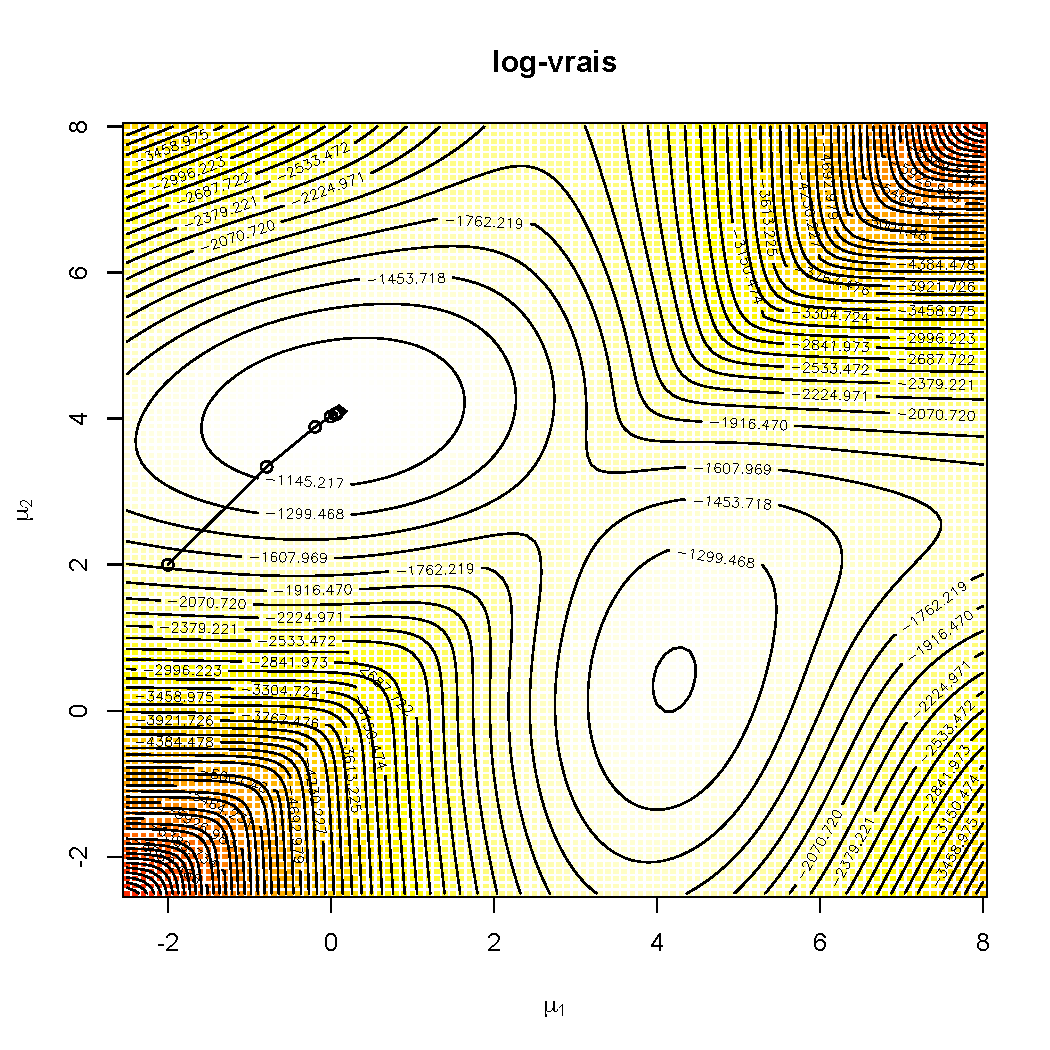
\includegraphics[width = 0.7 \textwidth]{figure-data_sim-logvrais-init1}
\end{frame}

%============================================
\begin{frame}{Illustration of the problems of convergence (II)}
%============================================
\centering
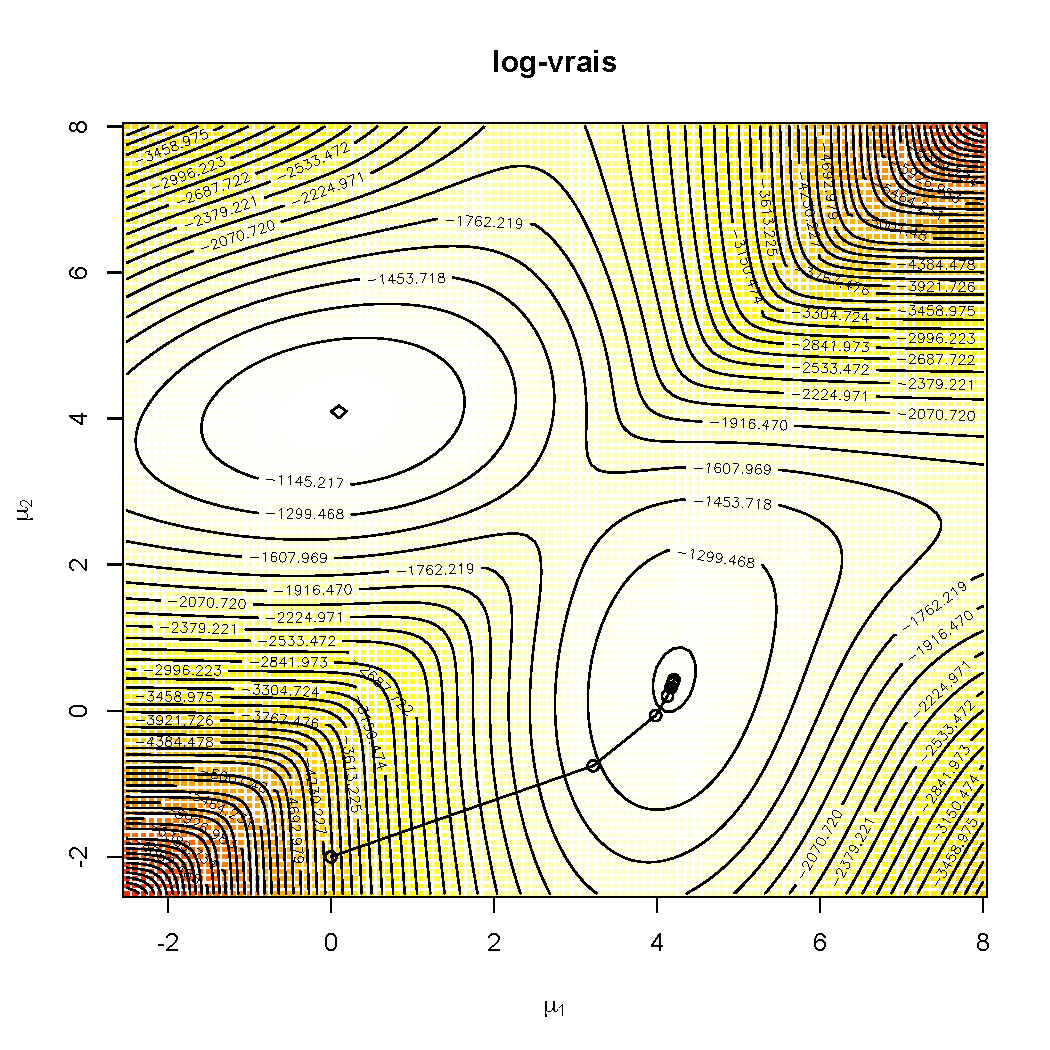
\includegraphics[width = 0.7 \textwidth]{figure-data_sim-logvrais-init2}
\end{frame}
%============================================
\begin{frame}{Illustration of the problems of convergence (III)}
%============================================
\centering
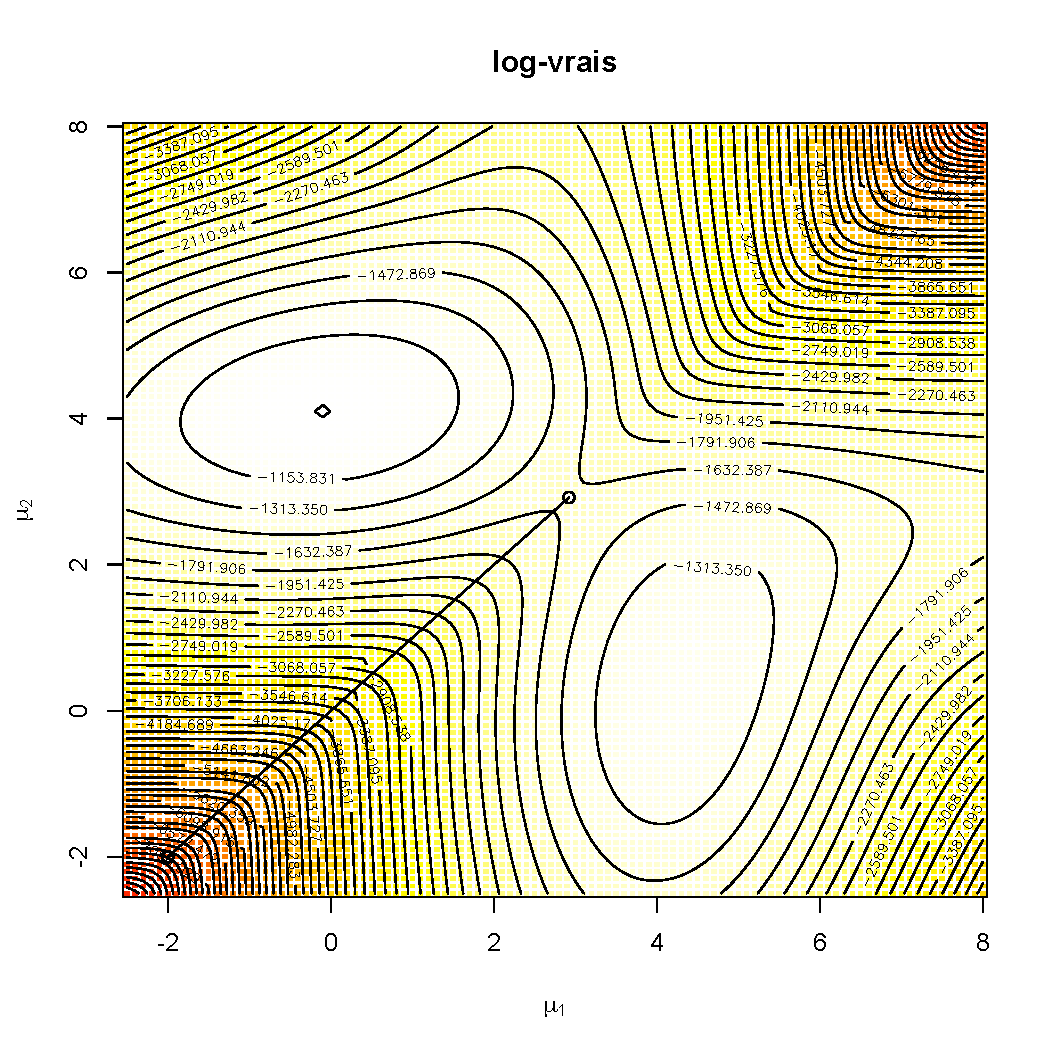
\includegraphics[width = 0.7 \textwidth]{figure-data_sim-logvrais-init3}
\end{frame}
 

 
%============================================
\begin{frame}{Application for the mixture model : E step}
%============================================
 
 E-step is straightforward for independent mixture models.
\label{Prop:LowerBound}
\begin{proposition} %
  In a mixture model \eqref{Eq:MixtureModel}, the hidden states $Z_i$ are independent conditional on the observations:
  $$
  p_\theta(\bZ|\bY) = \prod_{i=1}^n p_\theta(Z_i | Y_i)
  $$
  and, denoting $Z_{ik} = \mathbf{1}_{\{Z_i = k\}}$, the conditional distribution of each $Z_i$ is given by
  $$
  \tau_{ik} := P_\theta(Z_i = k | Y_i) = \Esp_\theta(Z_{ik} | Y_i) = \frac{\pi_k f_k(Y_i)}{\sum_{\ell = 1}^K \pi_\ell f_\ell(Y_i)}.
  $$
\end{proposition}
\end{frame}

%============================================
\begin{frame}[allowframebreaks]{Proof}
%============================================

\begin{itemize}
 \item First result is a direct consequence of Slide \ref{Rq:MixtureInd}
\item  Second result  follows from the Bayes formula

 
\begin{eqnarray*}
 \tau_{ik} &=& P_\theta(Z_i = k | Y_i) = \frac{P_\theta(Z_i = k) p_\theta(Y_i | Z_i = k)}{p_\theta(Y_i)} \\
 &=& \frac{P_\theta(Z_i = k) p_\theta(Y_i | Z_i = k)}{\sum_\ell P_\theta(Z_i = \ell) p_\theta(Y_i | Z_i = \ell)}.
\end{eqnarray*}

\item $P_\theta(Z_i = k | Y_i) = \Esp_\theta(Z_{ik} | Y_i)$   because $Z_{ik}$ is binary.
\end{itemize}


The update formula's of the $\tau_{ik}$ at the ($h+1$)-th E-step is then
$$
\tau^{h+1}_{ik} = \frac{{\pi}^h_k f(Y_i; {\gamma}^h_k)}{\sum_\ell {\pi}^h_\ell f(Y_i; {\gamma}^h_\ell)}
$$
where $\theta^h$ stands for the current estimate of $\theta$ resulting from the $h$-th M step.

\end{frame}


%============================================
\begin{frame}{Remark}
%============================================
 
 
Conditional probability $\tau_{ik}$ is sometimes referred to as the \textbf{\color{dgreen}  posterior probability} for observation $i$ to belong to class $k$ (as opposed to the \textbf{\color{dgreen} prior probability} $\pi_k$). 

Again this phrase is misleading in a non-Bayesian context and 'conditional probability' should be preferred.
\end{frame}


%============================================
\begin{frame}{M-step for the mixture model}
%============================================

$$\theta^{h+1} = \arg\max_\theta \Esp_{\theta^h}[\log p_\theta(\bY, \bZ) |\bY]$$

We use Proposition~ on Slide \ref{Prop:MixtureLikelihoods} to get an explicit formula for this quantity
\begin{eqnarray*}
  \Esp_{\theta^h}[\log p_\theta(Y, Z) |Y] & = & \Esp_{\theta^h}\left[\sum_{i=1}^n \sum_{k=1}^K Z_{ik} [\log \pi_k + \log f(Y_i; \gamma_k)] |\bY\right] \\
  & = &\sum_{i=1}^n \sum_{k=1}^K \Esp_{\theta^h}(Z_{ik}|Y_i) [\log \pi_k + \log f(Y_i; \gamma_k)] \\
  & = & \sum_{i=1}^n \sum_{k=1}^K\tau_{ik}^h [\log \pi_k + \log f(Y_i; \gamma_k)]. 
\end{eqnarray*}

\centering Has to be maximized with respect to $\theta = (\bpi, \bgamma)$, the $\tau_{ik}$ being fixed

\end{frame}
%============================================
\begin{frame}[allowframebreaks]{Application for the mixture model : M step ($\bpi$)}
%============================================
\begin{equation}\label{eq:pihat}
\pi^{h+1}_k = \frac{1}{n} \sum_{i=1}^n \tau^h_{ik}
\end{equation}

Indeed: 

\begin{itemize}
 \item  Using the  Lagrange multiplier to take into account the constraint $  \sum_{k=1}^K \pi_k= 1$
\item $$  \frac{\partial}{\partial \pi_k} \left[
  \sum_{i=1}^n \sum_{k=1}^K\tau_{ik}^h [\log \pi_k + \log f(Y_k; \gamma_k)] - \lambda \left(\sum_{k=1}^K \pi_k-1\right)\right] = 0 $$ 
  \item Leads to 
  $ \sum_{i=1}^n \frac{\tau_{ik}^h}{\pi_k^{h+1}} -\lambda = 0$ and so $\pi_k^{h+1} =  \frac{1}{\lambda}\sum_{i=1}^n\tau_{ik}^h$
\item  Moreover $  \sum_{k=1}^K \pi^{h+1}_k= 1$. So $ \frac{1}{\lambda}\sum_{k=1}^K \sum_{i=1}^n\tau_{ik}^h = \frac{1}{\lambda}\sum_{i=1}^n\underbrace{\sum_{k=1}^K \tau_{ik}^h}_{=1} = n$. 
\item Which implies Formula \eqref{eq:pihat}
 
\end{itemize}
 

 
 
 
 
  
\end{frame}


 %============================================
\begin{frame}{Application for the mixture model : M step ($\bgamma$)}
%============================================
 \begin{itemize}
 \item For $\bgamma$ : solution of this optimization problem has no general form as it strongly depends on the model at hand
\item Some general formula can be derived in the case of the  exponential family, as we will see in Slide   \ref{Slide:MixtureExpFam}
 \end{itemize}

\end{frame}



% 
% %============================================
% \begin{frame}{A Variational interpretation}
% %============================================
% \label{Sec:EM-VariatInterp}
% \begin{itemize}
%  \item A more general view on the EM algorithm and its extensions is given by the following property. 
%  \item Will be useful in the next chapters
% \end{itemize}
% 
% \begin{block}{Kullback-Leibler divergence}
% \begin{itemize}
%  \item Between distributions $q$ and $p$:
% \item   $	
%   \KL[q(Z)||p(Z)] = \Esp_q \{\log\left[q(Z) / p(Z)\right]\}
% $	
% \item  Always positive  
% because 
% \begin{eqnarray*}
% \Esp_q \log(q/p) &=& -\Esp_q \log(p/q)\\
% &\leq& - \log \Esp_q (p/q) \\
% &=& - \log \int p = - \log(1) = 0 
% \end{eqnarray*}
% 
% \item Null iff $q = p$. 
% \end{itemize}
% \end{block}
% 
% \end{frame}
% %============================================
% \begin{frame}{A Variational interpretation}
% %============================================
% 
% The following proposition gives a lower bound of the log-likelihood.
% \label{Prop:LowerBound}
% \begin{proposition}
% For any distribution $q$ on $\bZ$, we have
% $$
% \log p_\theta(\bY) \geq \Esp_q [\log p_\theta(\bY, \bZ)] + \Hcal[q(\bZ)].
% $$
% \end{proposition}
% 
% Because
% \begin{eqnarray*}
% \log p_\theta(\bY) & \geq & \log p_\theta(\bY) - \KL[q(\bZ)||p_\theta(\bZ|Y)] \\
%   & = & \log p_\theta(\bY) - \Esp_q [\log q(\bZ) - \log p_\theta(\bY, \bZ) + \log p_\theta(\bY)] \\
%   & = & \log p_\theta(\bY) - \Esp_q[\log q(\bZ)] + \Esp_q[\log p_\theta(\bY, \bZ)] - \underbrace{\Esp_q [\log p_\theta(\bY)]}_{\log p_\theta(\bY)}
% \end{eqnarray*}
% 
% \end{frame}
% 
%  
% %============================================
% \begin{frame}{Remark}
% %============================================
% 
% The decomposition given by Proposition~\ref{Prop:DecompLogLike} is similar to the lower bound of Proposition~\ref{Prop:LowerBound} with an equality when taking $q( \bZ) = p( \bZ|\bY)$. Furthermore, the E step of the EM algorithm can be viewed as the solution of the variational problem:
% $$
% q^*( \bZ) = \arg\min_q \KL[q( \bZ)||p( \bZ|\bY)],
% $$
% which, in absence of restriction for $q$ is $q^*( \bZ) = p( \bZ|\bY)$. From this point of view, the EM algorithm alternates the minimi zation of $KL[q( \bZ)||p( \bZ|\bY)]$ wrt $q$ (E step) and the maximization of the lower bound $\Esp_q [\log p_\theta(\bY,  \bZ)] + H[q( \bZ)]$ wrt $\theta$ (M step).
% \end{frame}

%============================================
\subsubsection{Case of the exponential family}
%============================================
\begin{frame}{Exponential family}\label{Slide:MixtureExpFam}
 
\label{Def:ExponFam}
\begin{definition}[Exponential family of distributions] 
  The distribution $f(;\gamma)$ belongs to exponential family with {\em canonical parameter} $\gamma$ if
  \[
  f(y;\gamma) = \exp[\gamma^\intercal t(y) - a(y) - b(\gamma)]
  \]
  where $t(y)$ is the vector of the {\em sufficient statistics}.
\end{definition}
\end{frame}

%============================================
\begin{frame}{Maximum likelihood for the exponential family}
%============================================
\label{Prop:ExpFam-bprime}
Two general properties that show connections between maximum likelihood estimates and moment estimates for this class of distribution. 

\begin{proposition} 
$b'(\gamma) = \Esp_\gamma[t(Y)]$.
\end{proposition}

\begin{proposition}
  For an iid sample $(Y_1, \dots Y_n)$, the MLE $\widehat{\gamma}$ of $\gamma$ satisfies 
  \[
  b' (\widehat{\gamma}) = \frac{1}{n}\sum_{i=1}^n t(Y_i) =: \overline{t}(Y).
  \] 
\end{proposition}
This shows that the MLE $\widehat{\gamma}$ is also the moment estimate of $\gamma$ based on the mean of the sufficient statistics.

{\scriptsize 
Proof in appendix slides \ref{app:proof1} and  \ref{app:proof2}.
}
\end{frame}


%============================================
\begin{frame}{EM for the exponential family}
%============================================


\begin{proposition}
  If all emission distributions $\Fcal_k$ belong to the exponential family with respective sufficient statistics $t_k$ and normalizing functions $a_k$ and $b_k$,
%  have the same form (i.e. share the same functions $t$, $a$ and $b$), 
  the maximization in the M step results in the weighted moment estimates based on the expectation of the sufficient statistics, i.e. ${\gamma}^{h+1}_k$ satisfies:
  $$
  \Esp_{{\gamma}^{h+1}_k}[t_k(U)] = \frac{T^{h+1}_k}{N^{h+1}_k}
  $$
  where 
  \begin{itemize}
   \item $U \sim f(\cdot, {\gamma}^{h+1}_k)$,
   \item $\tau^{h+1}_{ik} = \Esp_{{\theta}^{h+1}}[Z_{ik} | Y_i]$, 
   \item $N^{h+1}_k = \sum_{i=1}^n \tau^{h+1}_{ik}$
   \item  and $T^{h+1}_k = \sum_{i=1}^n\tau^{h+1}_{ik} t_k(Y_i)$.
  \end{itemize}
 
  
\end{proposition}
\end{frame}
%============================================
\begin{frame}[allowframebreaks]{Proof}
%============================================

Complete-likelihood for exponential family
\begin{eqnarray*}
 \log p_\theta(Y, Z) 
&=& \sum_{i=1}^n \sum_{k=1}^K Z_{ik} [\log \pi_k + \log f_k(Y_i)]\\
&=& \sum_{i=1}^n\sum_{k=1}^K Z_{ik} [\log \pi_k + \gamma_k^\intercal  t_k(Y_i) - a_k(Y_i) - b_k(\gamma_k)]
\end{eqnarray*}
 
So  conditional expectation is 
{\small \begin{eqnarray*}
&&\Esp[\log p_\theta(Y, Z) | Y]  = \\
&=& \Esp\left[\sum_{i=1}^n \sum_{k=1}^K Z_{ik} \left[\log \pi_k - b_k(\gamma_k)\right] | Y \right] + \Esp\left[\sum_{i=1}^n \sum_{k=1}^K Z_{ik} \left[\gamma_k^\intercal  t_k(Y_i) - a_k(Y_i)\right] | Y\right] \\
& = & \sum_{k=1}^K N_k [\log \pi_k - b_k(\gamma_k)] + \sum_{k=1}^K \gamma_k^\intercal  T_k - \sum_{i=1}^n \tau_{ik} a_k(Y_i).
\end{eqnarray*}

The derivative with respect to $\gamma_k$ is null iff $b_k'(\gamma_k) = T_k / N_k$ and the result follows from the general properties of the exponential family given in Propositions slide  \ref{Prop:ExpFam-bprime}.
}


\end{frame}

%============================================
\begin{frame}{Remarks}
%============================================


\begin{itemize}
 \item $\frac{T^{h+1}_k}{N^{h+1}_k}$ is an empirical weighted moment of the $Y_i$ 
 \item So the estimate of $\gamma_k$ resulting from Proposition slide \ref{Prop:ExpFam-bprime} is a moment-type estimate
 \item Depending on the form of $\Esp_{\gamma_k}[t_k(U)]$ as a function of $\gamma_k$, this estimate can have a close form or not
 
\end{itemize}
\end{frame}


%============================================
\begin{frame}{Expression for some popular models}
%============================================
\begin{itemize}
 \item \textcolor{dgreen}{Poisson mixture}: $\Fcal_k = \Pcal(\gamma_k)$:
  $$
  \widehat{\gamma}_k = \frac{1}{N_k} \sum_{i=1}^n \tau_{ik} Y_i. 
  $$
 \item \textcolor{dgreen}{Gaussian mixture}: $\Fcal_k = \Ncal(\mu_k, \sigma^2_k)$:
  $$
  \widehat{\mu}_k = \frac{1}{N_k} \sum_{i=1}^n \tau_{ik} Y_i, 
  \qquad
  \widehat{\sigma}^2_k = \frac{1}{N_k} \sum_{i=1}^n \tau_{ik} (Y_i - \widehat{\mu}_k)^2.
  $$	
 \item \textcolor{dgreen}{Multinomial mixture}: $\Fcal_k = \Mcal(1; \gamma_k)$, denoting $Y_{ia} = \Ibb_{\{Y_i = a\}}$:
  $$
  \widehat{\gamma}_{ka} = \frac{1}{N_k} \sum_{i=1}^n \tau_{ik} Y_{ia}. 
  $$	
\end{itemize}

\end{frame}

%============================================
\begin{frame}{About the entropy}
%============================================

$$\Hcal[p_\theta(\bZ|\bY)]  = -\Esp_{\theta}[\log p_\theta(\bZ | \bY) | \bY]$$ 

Can be calculated using the conditional independence of the $Z_i$ given the data $\bY$:
\begin{eqnarray} \label{Eq:MixtureEntropy}
  \Hcal[p_\theta(\bZ|\bY)] & = & \sum_{i=1}^n H[p_\theta(Z_i|Y_i)] \nonumber \\
    & = & - \sum_{i=1}^n \Esp_\theta[\log P(Z_i = k|Y_i) | Y_i] \\
    & = & - \sum_{i=1}^n \sum_{k=1}^K \tau_{ik} \log \tau_{ik}. \nonumber 
\end{eqnarray}


\end{frame}


%============================================
\subsubsection{Asymptotic variance and Fisher information}
%===========================================


%============================================
\begin{frame}{Fisher information and asymptotic variance of the ML}
%============================================

Asymptotic variance of the maximum likelihood estimate
$$
\widehat{\theta} = (\widehat{\bpi}, \widehat{\bgamma})
$$
is provided by the Fisher information matrix $I$ by
$$
\Var_{\infty}(\widehat{\theta}) = I_\theta^{-1}
$$
where
\begin{eqnarray*}
 S_\theta(Y) &=& \partial_\theta \log p_\theta(Y)\\
I_\theta &=& \Esp_Y[S_\theta(Y) S_\theta(Y)^{\intercal}]
 = - \Esp_{Y}\left[\partial^2_{\theta^2} \log p_\theta(Y)\right]\\
 &=& -\Esp_{Y}\left[S'_\theta(Y)\right]
\end{eqnarray*}
 
 \textcolor{dgreen}{Problem}: Evaluation of $S'_\theta(Y)  = \partial^2_{\theta^2} \log p_\theta(Y)$ because $p_\theta(Y)$ is a sum. 
\end{frame}

%============================================
\begin{frame}[allowframebreaks]{Louis's formula}
%============================================
 \label{Prop:Louis}
\cite{Louis82} provides a convenient way to compute the Hessian matrix
$$
S_\theta'(Y) = \partial^2_{\theta^2} \log p_\theta(Y),
$$
which only uses by-products of the EM algorithm. 

\begin{proposition}[\cite{Louis82}]
\begin{eqnarray*}
   S_\theta'(Y) &=& \Esp[S_\theta'(Y ,Z) | Y] +  \Esp\left[S_\theta(Y, Z) S_\theta(Y, Z)^\intercal | Y \right]\\
   && - \Esp[S_ \theta(Y, Z) | Y] \Esp[S_ \theta(Y, Z) | Y]^\intercal.
\end{eqnarray*}
\end{proposition}

{Proof is given in Appendix on Slide \ref{App:AssVar}.}
\vspace{3em}

\textcolor{dgreen}{Two main interests}:
\begin{itemize}
\item Involve the complete likelihood and can, most of
  the times, be easily computed (see example in Apppendix Slide  \ref{App:AssVarPoiss})  
\item Last term null  when $\theta = \widehat{\theta} =
  \arg\max \log p_\theta(Y)$. 
  
  Indeed (see the proof Slide \ref{App:AssVar})
  $$\Esp[S_ \theta(Y, Z) | Y] = S_\theta(Y) =\frac{p'_\theta(Y)}{p_\theta(Y)}$$  which is equal to $0$ for  $\theta = \widehat{\theta}$
  since $\left.p_\theta'(Y)\right|_{\widehat{\theta}} = 0$.
\end{itemize}
\end{frame}

%============================================


%============================================
\subsection{Choosing $K$}
%============================================
\begin{frame}{How many states?}
%============================================ 
\begin{itemize}
 \item $K$ is not known general
 \item A model with $K-1$ classes is nested in a model with $K$ classes : the likelihood increases as well
 \item Likelihood not a relevant criterion to estimate $K$
\item Dimension of the parameter $\theta$ increases with $K$.
\end{itemize}
  
  
  \begin{center}
   \textcolor{dgreen}{Penalized likelihood criteria}
  \end{center}

  
\end{frame}

%============================================
\begin{frame}{Penalized likelihood criterion}
%============================================ 


\begin{itemize}
 \item Let $\widehat{\theta}_K$ be the maximum likelihood estimate of $\theta$ for a model with $K$ components:
$$
\widehat{\theta}_K = \arg\max_{\theta \in \Theta_K} \log p_\theta(\bY)
$$
where $\Theta_K$ :  parameter space for a $K$-mixture model
\item \textcolor{dgreen}{Penalized likelihood estimate of $K$}: 
$$
\widehat{K} = \arg\max_K \left(\log p_{\widehat{\theta}_K}(\bY) - \text{pen}(K)\right).
$$ 
\end{itemize}
\end{frame}

%============================================
\begin{frame}{Bayesian information criterion}
%============================================ 

\begin{itemize}
 \item Most commonly used criterion \cite{Schwarz78}
 \item Originally defined in a Bayesian framework
\end{itemize}
Three levels of hierarchy:
\begin{enumerate}
 \item a prior distribution $p(K)$ for the number of components;
 \item a conditional distribution $p(\theta|K)$ for the parameter $\theta$ given the number of components;
 \item a likelihood $p_\theta(\bY)$ which corresponds to the conditional distribution of the observations $Y$ given the parameters: $p_\theta(\bY) = p(\bY | \theta, K)$.
\end{enumerate}
\end{frame}

%============================================
\begin{frame}{Posterior probability of $K$}
%============================================ 

\begin{itemize}
 \item Model selection problem relies on conditional distribution of $K$ given the observations:
$$
p(K|\bY) = \frac{p(Y, K)}{p(\bY)} = \frac{p(K) p(\bY|K)}{p(\bY)}.
$$
\item 
Ideally, one would choose
\begin{eqnarray*}
\widehat{K} & = & \arg\max_K \; p(K|\bY) \; = \; \arg\max_K \; \left(\log p(K) + \log p(\bY| K)\right) \\
%  & = & \arg\max_K \; \left(\log p(K) + \log \int p(Y|\theta , K) p(\theta|K) \dd \theta\right).
\end{eqnarray*}
\item But 
$ \log p(Y| K) = \log \int p(\bY|\theta , K) p(\theta|K) \dd \theta$

\begin{itemize}
\item Difficult to evaluate 
\item Laplace approximation 
\end{itemize}
\end{itemize}
\end{frame}
%============================================
\begin{frame}{Laplace approximation}
%============================================ 

\begin{proposition}[Laplace approximation]
Under regularity conditions,
$$
\log p(\bY | K) = \log p_{\widehat{\theta}_K}(\bY) - \frac{d_K}2 \log n + \mathcal{O}_n(1).
$$
where $d_K$ denotes the number of independent parameters in a model with $K$ components.
\end{proposition}

\begin{itemize}
 \item Detailed proof:  \cite{Lebarbier04}, together with precise comparative study between BIC and another popular model selection criterion: AIC.
 \item The term $\log p(K)$ remains fix when $n$ grows large: neglected
\end{itemize}

\end{frame}


%============================================
\begin{frame}{BIC}
%============================================ 

\begin{definition}
 $$
  \widehat{K}_{BIC} = \arg\max_K \left(\log p_{\widehat{\theta}_K}(\bY) - \frac{d_K}2 \log n\right).
  $$ 
\end{definition}

\end{frame}

%============================================
\begin{frame}{From BIC to Integrated Complete Likelihood (ICL)}
%============================================ 



Using Proposition \ref{Prop:DecompLogLike}
$$
\log p_{\widehat{\theta}_K}(\bY) = 
\Esp_{\widehat{\theta}_K} \left[\log p_{\widehat{\theta}_K}(\bY, \bZ) | \bY\right] - \underbrace{\Esp_{\widehat{\theta}_K} \left[\log p_{\widehat{\theta}_K}(\bZ |\bY)|\bY\right]}_{\color{dgreen}(1)}
$$

\begin{itemize}
\item $\color{dgreen}(1)$: entropy of the classification distribution
\item Entropy is small when the observations are classified with reasonable confidence.

\item \cite{biernacki2000}: account for the classification uncertainty in the selection of $K$
\item Penalize value of $K$ with large entropy
\end{itemize}
 \end{frame}

%============================================
\begin{frame}{ICL}
%============================================ 
\begin{definition}[ICL]
\begin{eqnarray*}
  \widehat{K}_{ICL} &=& \arg\max_K \left(\log p_{\widehat{\theta}_K}(Y) - \Hcal[p_{\widehat{\theta}_K}(\bZ | \bY)]- \frac{d_K}2 \log n\right)\\
  &=& \arg\max_K \left(\Esp_{\widehat{\theta}_K} \left[\log p_{\widehat{\theta}_K}(\bY, \bZ) | \bY\right] - \frac{d_K}2 \log n\right)
\end{eqnarray*}
\end{definition}

\end{frame}


% 
% \paragraph{Illustration.} 
% The following figures illustrate the behavior of this two criteria for the nematode gene expression data (Ex. \ref{Ex:NematodeGeneExp}). We see that BIC favors the fit to the marginal distribution of the observation, whereas ICL favors the separation between the components.
% 
% 
% \begin{figure}[H]
%  \begin{center}
%   \includegraphics[width=0.5\textwidth]{../Figures/26-AT2G38940-BICICL}
%   \caption{BIC and ICL criteria for the choice of a Gaussian mixture model for the nematode gene expression data as a function of the number of groups $K$. $\triangle:$ equal variances, $\textcolor{blue}{\triangledown}:$ heterogeneous variances. Solid lines: BIC, dashed lines: ICL. (same data as in Fig.~\ref{Fig:NematodeGeneExp})}
%  \end{center}
% \end{figure}
% 
% \begin{figure}[H]
%  \begin{center}
%   \begin{tabular}{cc}
%   \includegraphics[width=0.4\textwidth]{../Figures/26-AT2G38940-homoBIC} &
%   \includegraphics[width=0.4\textwidth]{../Figures/26-AT2G38940-homoICL} \\
%   \end{tabular}
%   \caption{Comparison of the homogeneous variance mixture models selected with BIC (left) and ICL (right) for the nematode gene expression data. (same data as in Fig.~\ref{Fig:NematodeGeneExp})}
%  \end{center}
% \end{figure}
% 
% \begin{figure}[H]
%  \begin{center}
%   \begin{tabular}{cc}
%   \includegraphics[width=0.4\textwidth]{../Figures/26-AT2G38940-heteroBIC} &
%   \includegraphics[width=0.4\textwidth]{../Figures/26-AT2G38940-heteroICL} \\
%   \end{tabular}
%   \caption{Comparison of the heterogeneous variance mixture models selected with BIC (left) and ICL (right) for the nematode gene expression data. (same data as in Fig.~\ref{Fig:NematodeGeneExp})}
%  \end{center}
% \end{figure}

 
%============================================
\subsection{Classification} \label{Subsec/ MixtClassif}
%============================================
\begin{frame}{Unsupervised classification}
%============================================
 \begin{itemize}
  \item Often the main aim when using a mixture model. 
  \item Maximum likelihood inference provides estimates of  $\theta$
  \item By-product of EM : conditional distribution of the hidden classes $\bZ$ conditional to the observed data $\bY$
\end{itemize}
\end{frame}
%============================================
\begin{frame}{Soft classification}
%============================================
$$\tau_{ik} = P_{\widehat{\theta}}(Z_i = k | \bY)$$
 \begin{itemize}
  \item Gives a measure of the confidence with which an observation could be classified into a given group
\item Uncertainty of the classification   summarized by: 
$$
\Hcal[p_{\widehat{\theta}}(Z_i|\bY)] = \Hcal[p_{\widehat{\theta}}(Z_i|Y_i)] = - \sum_{k=1}^K \tau_{ik} \log \tau_{ik}.
$$
Sometimes referred to as the {\sl classification uncertainty}
\item Entropy of the whole conditional distribution of $Z$  given $Y$: sum of all the individual's uncertainties
\end{itemize}  
\end{frame}
%============================================
\begin{frame}{Hard classification}

When observations need to be classified into groups, the most common rule is the 'maximum a posteriori' (MAP) rule.

\begin{definition} \label{Def:MAP}
 The MAP classification rule is given by:
$$
\widehat{\bZ} = \arg\max_z p_\theta(\bZ=z | \bY).
$$
\end{definition}

 
\begin{itemize}
 \item The MAP rule can be applied to each observation label $Z_i$ as
$$
\widehat{Z}_i = \arg\max_k \tau_{ik}
$$
\item In the case of mixture, equivalent:
$$
\widehat{\bZ} = \arg\max_\bz p_\theta(\bZ=\bz | \bY) = (\widehat{Z}_i)_i
$$
since the $Z_i$ are independent conditionally on $\bY$.
\end{itemize}
 
\end{frame}


%============================================
\begin{frame}{Conclusion}
 
\begin{itemize}
 \item Idea really simple. 
 \item Example of \textsf{R} package : mixtools
 \item Used in many context, even for complexe data. The emission distribution has to be adapted. 
 \item Next chapter : Hidden Markov Models
\end{itemize}
 
 
\end{frame}


%============================================


%============================================
\begin{frame}{References}
\bibliographystyle{apalike}
 \bibliography{/home/donnet/Dropbox/WORK_DROPBOX/ENSEIGNEMENT/2024-Saclay-MathsSV/CoursVariablesLatentes/LVM_CoursComplet/tools/biblioLVM}
\end{frame}


%===============================================
\begin{frame}[allowframebreaks]{Appendix. Properties of the exponential family}
\label{app:proof1}

\begin{proposition} 
$b'(\gamma) = \Esp_ \gamma[t(Y)]$.
\end{proposition}

Remind that the moment generating function of   $V$
$$m(z) = \Esp[e^{z^\intercal V}]$$ with
$m'(0) = \Esp(V)$

For the exponential family, consider the moment generating function of the sufficient statistics  
\begin{eqnarray*}
 m(z) &:=& \Esp[e ^{z^\intercal  t(Y)}] = \int e^{z^\intercal  t(y)} f_\gamma(y) \dd y \\
&=& \int \exp[(z + \gamma)^\intercal  t(y) - a(y) - b(\gamma)] \dd y.
\end{eqnarray*}

Because $f_\gamma$ is a pdf, $e^{b(\gamma)}$ is a normalizing constant:
\begin{eqnarray*}
\int \exp[\gamma^\intercal  t(y) - a(y)] \dd y & = & e^{b(\gamma)} \\
\Rightarrow \qquad \int \exp[(z + \gamma)^\intercal  t(y) - a(y)] \dd y & = & e^{b(z +\gamma)} 
\end{eqnarray*}
so
$$
m(z) = e^{-b(\gamma)} \int \exp[(z + \gamma)^\intercal  t(y) - a(y)] \dd y 
= e^{b(z + \gamma) - b(\gamma)}.
$$ 
The result follows from the fact that $m'(z) = b'(\gamma+z) \Rightarrow m'(0) = b'(\gamma)$.
\hyperlink{Prop:ExpFam-bprime}{\beamerreturnbutton{Go back to the course}}


\end{frame}
%===========================================
\begin{frame}[allowframebreaks]{Appendix. Properties of the exponential family}
%===========================================
\label{app:proof2}
\begin{proposition}
  For an iid sample $(Y_1, \dots Y_n)$, the MLE $\widehat{\gamma}$ of $\gamma$ satisfies 
  \[
  b' (\widehat{\gamma}) = \frac{1}{n}\sum_{i=1}^n t(Y_i) =: \overline{t}(Y).
  \] 
\end{proposition}


Take the derivative of the log-likelihood 
\[
\sum_i \log p(Y_i; \gamma) = \sum_i [\gamma^\intercal t(Y_i) - a(Y_i)] - n b(\gamma)
\]
with respect to $\gamma$. 


\hyperlink{Prop:ExpFam-bprime}{\beamerreturnbutton{Go back to the course}}


\end{frame}
 
 
 
%===========================================
\begin{frame}[allowframebreaks]{Appendix. Asymptotic variance}
%===========================================

\label{App:AssVar}

\begin{proposition}[\cite{Louis82}]
\begin{eqnarray*}
   S_\theta'(Y) &=& \Esp[S_\theta'(Y, Z) | Y] +  \Esp\left[S_\theta(Y, Z) S_\theta(Y, Z)^\intercal | Y \right]\\
   && - \Esp[S_ \theta(Y, Z) | Y] \Esp[S_ \theta(Y, Z) | Y]^\intercal.
\end{eqnarray*}
\end{proposition}

\textbf{Demonstration}

Recalling that
$$
\log p_\theta(Y) = \log \left[\sum_z p_\theta(Y, z) \right], 
$$
we have
\begin{eqnarray}
  S_ \theta(Y)  & = & p_\theta'(Y) \left/ p_\theta(Y) \right. \; = \; \sum_z p'_\theta(Y, z) \left/ p_\theta(Y) \right. \nonumber \nonumber \\ 
  & = & \sum_z \frac{p'_\theta(Y, z)}{p_\theta(Y, z)} p_\theta(Y, z) \left/p_\theta(Y) \right.
  \; = \; \sum_z \frac{p'_\theta(Y, z)}{p_\theta(Y, z)} p_\theta(z | Y) \nonumber \\
%   = \; \sum_{z} \underset{p_\theta(z| Y)}{\underbrace{\frac{p_\theta(Y, z)}{\sum_{z'}
%     p_\theta(Y, z')}}} \underset{S_ \theta(Y,  z)}{\underbrace{\frac{p_\theta'(Y, z)}{p_\theta(Y,z)}}} \\
%   & = & \sum_{z} p_\theta(z| Y) S_ \theta(Y, z) 
  & = & \Esp\left[\frac{\partial}{\partial \theta} \log p_\theta(Y, z) \right]  \; = \; \Esp[S_ \theta(Y, Z) | Y]. \label{Eq:LouisTrick}
\end{eqnarray} 
Because the second derivative of $\log f$ is 
\begin{equation} \label{Eq:Der2ndLog}
(\log f)'' = \frac{f''}{f} - \left(\frac{f'}{f}\right) \left(\frac{f'}{f}\right)^{\intercal}
\end{equation}
the second derivative of $\log p_\theta(Y)$ is
%\begin{eqnarray*}
% S_\theta'(Y) & = & \frac{\partial^2}{\partial \theta^2} \log \sum_z p_\theta(Y, z) \\
%    & = & \frac{\sum_z p_\theta''(Y, z)}{p_\theta(Y)} - \left[\frac{\sum_z p_\theta'(Y, z)}{\sum_z p_\theta(Y, z)}\right] \left[\frac{\sum_z p_\theta'(Y, z)}{\sum_z p_\theta(Y, z)}\right]^\intercal \\
%  & = & \frac{\sum_z p_\theta''(Y, z)}{p_\theta(Y)} - \Esp[S_ \theta(Y, Z) | Y] \Esp[S_ \theta(Y, Z) | Y]^\intercal.
%\end{eqnarray*}

\begin{eqnarray*}
 S_\theta'(Y) & = & \frac{\partial^2}{\partial \theta^2} \log p_\theta(Y) \\
& = & \frac{p_\theta''(Y)}{p_\theta(Y)} - \left[\frac{p_\theta'(Y)}{p_\theta(Y)}\right]\left[\frac{p_\theta'(Y)}{p_\theta(Y)}\right]^\intercal \\
 & = & \frac{\sum_z p_\theta''(Y, z)}{p_\theta(Y)} - \Esp[S_ \theta(Y, Z) | Y] \Esp[S_ \theta(Y, Z) | Y]^\intercal.
\end{eqnarray*}

% $$
% S_\theta'(Y) = \frac{p_\theta''(Y)}{p_\theta(Y)}
% - \left[\frac{p_\theta'(Y)}{p_\theta(Y)} \right]
% \left[\frac{p_\theta'(Y)}{p_\theta(Y)} \right]^{\intercal};
% $$
The same trick as in \eqref{Eq:LouisTrick} can be combines with \eqref{Eq:Der2ndLog} for the first term to get
{\scriptsize \begin{eqnarray*}
 \frac{\sum_z p_\theta''(Y, z)}{p_\theta(Y)}  
  & = & \sum_z \left[\frac{p_\theta''(Y, z)}{\color{orange}p_\theta(Y, z)} 
  - \left(\frac{p_\theta'(Y, z)}{p_\theta(Y, z)}\right) \left(\frac{p_\theta'(Y, z)}{p_\theta(Y, z)}\right)^\intercal 
  + \left(\frac{p_\theta'(Y, z)}{p_\theta(Y, z)}\right) \left(\frac{p_\theta'(Y, z)}{p_\theta(Y, z)}\right)^\intercal \right] \\
  && \quad \quad \quad  \times \underbrace{\frac{\color{orange}p_\theta(Y, z)}{p_\theta(Y)} }_{=p_\theta(Z| \bY)}\\	
  & = & \sum_z \left[\frac{\partial^2}{\partial \theta^2}  \log p_\theta(Y, z)
  + \left(\frac{p_\theta'(Y, z)}{p_\theta(Y, z)}\right) \left(\frac{p_\theta'(Y, z)}{p_\theta(Y, z)}\right)^\intercal \right] p_\theta(z|Y) \\
  & = &  \Esp[S_\theta'(Y, Z) | Y] +  \Esp\left[S_\theta(Y, Z) S_\theta(Y, Z)^\intercal | Y\right]
\end{eqnarray*}}
which completes the proof. 


\hyperlink{Prop:Louis}{\beamerreturnbutton{Go back to the course}}


\end{frame}
 
%===========================================
\begin{frame}[allowframebreaks]{Appendix 2: Assymptotic variance for the Poisson emission distribution}
%===========================================
\label{App:AssVarPoiss}
%============================================

 \begin{itemize}
  \item Mixture model \eqref{Eq:MixtureModel} where $F(\gamma_k) = \Pcal(\gamma_k)$. 
  \item Complete log-likelihood
$$
\log p_\theta(Y, Z) = \sum_{i, k} Z_{ik} \left[\log \pi_k - \gamma_k + Y_i \log \gamma_k - \log (Y_i!) \right]
$$
where $\pi_K = 1- \sum_{k < K} \pi_k$. 

\item First derivatives 
 \begin{itemize}
\item $\partial_{\pi_k} \log p_\theta(Y, Z) = \frac{\sum_{i=1}^n Z_{ik}}{\pi_k} - \frac{\sum_{i=1}^n Z_{iK}}{\pi_K}$
\item $\partial_{\gamma_k} \log p_\theta(Y, Z) = -\sum_{i=1}^n Z_{ik} + \frac{\sum_{i=1}^n Z_{ik} Y_i}{\gamma_k} 
$
\end{itemize}
\framebreak
\item Second derivatives:
\begin{itemize}
\item $
\partial^2_{\pi_k^2} \log p_\theta(Y, Z) = -\frac{\sum_{i=1}^n Z_{ik}}{\pi_k^2} + \frac{\sum_{i=1}^n Z_{iK}}{\pi_K^2}, 
$
\item $
\partial^2_{\pi_k, \pi_\ell} \log p_\theta(Y, Z) = \frac{\sum_{i=1}^n Z_{iK}}{\pi_K^2}
$
\item $
\partial^2_{\gamma_k^2} \log p_\theta(Y, Z) = -\frac{\sum_{i=1}^n Z_{ik} Y_i}{\gamma_k^2},
$
\item $\partial^2_{\gamma_k, \gamma_\ell} \log p_\theta(Y, Z) = 0.
$
\end{itemize}
\end{itemize}

The first term of Prop slide ~\ref{Prop:Louis} requires the calculation of the following moments, denoting here $\Esp^Y(\cdot) = \Esp(\cdot | Y)$:
$$
\begin{array}{rcl}
  \Esp^Y\left( \sum_{i=1}^n Z_{ik} \right) & = & \sum_{i=1}^n \tau_{ik} =: N_k, \\
  \Esp^Y\left( \sum_{i=1}^n Z_{ik} Y_i \right) & = & \sum_{i=1}^n \tau_{ik} Y_i =: S_k. \\
\end{array}
$$
The second term requires these of



$$
\begin{array}{rcl}
%\begin{eqnarray*}
 \Esp^Y\left[\left(\sum_{i=1}^n Z_{ik} \right) \left(\sum_{i=1}^n Z_{i\ell} \right) \right] &=&  
 \Esp^Y\left(\sum_{i=1}^n Z_{ik} Z_ {i\ell}  + \sum_{i \neq j} Z_{ik} Z_ {j\ell} \right) \\
  &=&  \sum_{i=1}^n \Esp^Y(Z_{ik} Z_ {i\ell})\\
  && + \sum_{i \neq j} \Esp^Y(Z_{ik}) \Esp^Y(Z_{j\ell}) \\ 
 &=^*&  \sum_{i=1}^n  \mathbf{1}_{\{k=\ell\}}  \tau_{ik} + \sum_{i \neq j} \tau_{ik} \tau_{j\ell} \quad \\
 &=& \quad \mathbf{1}_{\{k=\ell\}}  N_k+ N_k N_\ell - \sum_{i=1}^n \tau_{ik} \tau_{i\ell}, \\
  \Esp\left[\left(\sum_{i=1}^n Z_{ik} Y_i \right) \left(\sum_{i=1}^n Z_{i\ell} \right) \right] 
  &=&  \mathbf{1}_{\{k=\ell\}}  S_k + S_k N_\ell - \sum_{i=1}^n Y_i \tau_{ik} \tau_{i\ell}, \\
 \Esp^Y\left[\left(\sum_{i=1}^n Z_{ik} Y_i \right) \left(\sum_{i=1}^n Z_{i\ell} Y_i \right) \right] 
   &=&  \mathbf{1}_{\{k=\ell\}}  Q_k + S_k S_\ell - \sum_{i=1}^n Y_i^2 \tau_{ik} \tau_{i\ell}, \\
%\end{eqnarray*}
\end{array}
$$
where $Q_k = \sum_{i=1}^n Y_i^2 \tau_{ik}$ and  $\;^*$ because  $Z_{ik} Z_{i\ell} = 0$ if $k \neq \ell$.

\hyperlink{Prop:Louis}{\beamerreturnbutton{Go back to the course}}

\end{frame}



\end{document}
